\documentclass{article}
\usepackage{graphicx} %for inserting image
\usepackage{float}
\setlength{\parindent}{20pt}
\usepackage[a4paper, margin=3cm]{geometry}
\usepackage[utf8]{inputenc}
\usepackage[T1]{fontenc}
\usepackage[french]{babel}
\usepackage{geometry}  
\usepackage{array}
\usepackage{hyperref}
\renewcommand{\arraystretch}{1.5} % Augmente l'espacement entre les lignes
\usepackage{multirow} % Pour aligner correctement les colonnes si besoin


\begin{document}
\begin{titlepage}
    \centering
    \vspace*{\fill}

    {\Huge \textbf{Software Requirements Document:}\\[0.5cm]
    \textbf{Tetris Royal}} \\[1.5cm]
    
    {\Large Tao Chau\\
    Juliete Cornu-Besser\\
    Quentin Bernard Bouissières\\
    Jonas Schellekens\\
    Ethan Van Ruyskenvelde\\
    Lucas Verbeiren\\
    Ernerst Malysz\\
    Rafaou Gajewicz} \\[2cm]

    {\Large 13 décembre 2024}

    \vspace*{\fill} 
\end{titlepage}

\newpage

\tableofcontents

\newpage

\section{Introduction}

\subsection{But du projet}

\quad Ce projet a pour objectif de concevoir une application de jeu intégrant diverses fonctionnalités multijoueur. Les règles des parties reprendront celles existantes dans \textit{Tetris Royal}, une extension de la version normale du jeu \textit{Tetris}. Chaque joueur possède une grille vide qu'il doit essayer de remplir en laissant le moins d'espace possible avec des \textit{tetrominoes}, des formes géométriques qui peuvent être tournées et déplacées avant leur place finale. Les pièces tombent depuis le haut de la grille et plus la partie avance, plus elles tombent rapidement. Une ligne remplie de  \textit{tetrominoes} se supprime et fait gagner des points au joueur. La partie se termine quand le joueur ne sait plus placer de formes géométriques sur la grille car il y a des \textit{tetrominoes} sur toute la hauteur de la grille. Son score dépendra du temps de la partie et des lignes supprimées.  

\paragraph*{}

Dans cette application, quatre modes sont proposés au joueur. Il existe la version \textit{Endless} avec un seul joueur où le but est de savoir placer des pièces sur la grille le plus longtemps possible. Selon les combinaisons des pièces qui se suppriment, les points attribués seront différents.
 
\paragraph*{}

Puis nous implémenterons les modes multijoueurs. Une nouvelle notion doit être introduite : "\textit{une ligne de penalty}". Un joueur peut envoyer un penalty à un adversaire. Le receveur du penalty retrouvera toutes ses lignes poussées vers le haut pour laisser la place à une ou plusieurs rangées avec un bloc manquant en dessous, qui ne peuvent pas être supprimées par les combinaisons.  

\paragraph*{}

La version \textit{Classic} et la version \textit{Duel} comprennent respectivement des parties de trois à neuf, et de deux joueurs. Chaque participant a sa propre grille avec ses \textit{tetrominoes} qui tombent; celui qui complète une ou plusieurs lignes en même temps peut envoyer des lignes de penalty selon sa combinaison à un adversaire de son choix. 

\paragraph*{}

Le dernier mode, \textit{ Royal Competition}, comprend des penalties multiples et des bonus. Ce sont des parties de trois à neuf joueurs. Chaque individu aura sa propre barre d'énergie initialement nulle. Au fil de la partie, la barre se remplit selon les combinaisons de lignes supprimées du joueur. Une fois cette dernière atteignant une valeur, le joueur peut acheter des penalties pour les envoyer à un adversaire ou s'octroyer un bonus qui lui facilite la partie pendant une période donnée. Dans la liste étendue de penalties et de bonus, nous retrouvons un ralentissement de la chute des \textit{tetrominoes} pour soi-même, augmenter cette vitesse pour un adversaire ou encore inverser les commandes d'action d'un adversaire.

\paragraph*{}

En dehors des parties de jeux, le joueur peut se connecter ou créer un compte pour accéder au \textit{Tetris Royal}. Cela lui permet de gérer sa liste d'amis et de discuter avec eux via une messagerie intégrée à l'application. Il peut également consulter le classement des autres joueurs dans le mode \textit{Endless}. Pour terminer, il peut créer ou rejoindre une partie dans un mode multijoueur sélectionné. Les participants peuvent être invités en mode observateur ou en mode joueur.

\newpage

\subsection{Glossaire}


\begin{itemize}

    \item \textbf{Blackout} : Pénalité qui "éteint la lumière" chez un adversaire ( le joueur ne voit plus son tableau pendant un court moment)
    
	\item \textbf{Bonus} : Avantage obtenu par le joueur lorsque celui-ci dépense son énergie. Un bonus peut prendre plusieurs formes:

    \item \textbf{Effect} : terme regroupant les pénalités et les bonus utilisés dans le mode royal

    \item \textbf{InputLock} : Pénalité qui bloque les commandes d'un adversaire pour le prochain tetromino.

    \item \textbf{Lightning} : Pénalité qui envoie un eclair qui supprime des blocs dans une zone de 2 x 2 chez un adversaire.

    \item \textbf{Matchmaking} : Système qui permet de connecter plusieurs joueurs ensemble pour pouvoir créer et lancer une partie en ligne.
    
    \item \textbf{Mini Tetrominoes} : Avantage qui fait que les 2 prochains tetrominoes se transforment en bloc de 1 x 1.
    
	\item \textbf{Penalty} : Pénalité infligée à un joueur par un de ses adversaires. Le penalty se manifeste par l'ajout d'une ou de plusieurs lignes supplémentaires en bas de la grille du receveur, poussant les blocs existants vers le haut et rapprochant le joueur de la défaite. Cette ligne de pénalité peut être supprimé de la grille si le joueur arrive à compléter avec ses tetrominoes. 
    
    \item \textbf{Slow Down} : Avantage qui réduit la vitesse de chute des tetrominoes sur ton plateau.

    \item \textbf{Speed Up} : Pénalité qui augmente la vitesse de chute des tetrominoes sur le plateau d'un adversaire.

    \item \textbf{Reverse Controls} : Pénalité qui inverse les commandes d'un adversaire pour les trois prochaines tetrominoes.

    \item \textbf{Tetromino} : Pièce de jeu composée de quatre blocs carré connectés entre eux de manière à former différentes formes géométriques, respectivement (Z, L, O, S, I, J, T). 

    \item \textbf{Username} : Nom utilisé par un utilisateur et qui peut ne pas être son nom officiel.

\end{itemize}

\newpage

\subsection{Historique}


\begin{table}[h!]
    \centering
    \begin{tabular}{|>{\centering\arraybackslash}m{2cm}|>{\centering\arraybackslash}m{6cm}|>{\centering\arraybackslash}m{4cm}|>{\centering\arraybackslash}m{2cm}|}
        \hline
        \textbf{Numéro de version} & \textbf{Nom} & \textbf{Modifications} & \textbf{Date} \\
        \hline
        0.1 & Quentin Bernard Bouissières / Jonas Schellekens / Ethan Van Ruyskenvelde / Lucas Verbeiren & Besoins utilisateurs fonctionnels & 20/11/2024 \\ \hline
        0.2 & Juliette Cornu-Besser / Jonas Schellekens & Introduction + Glossaire + commentaires Besoin utilisateur & 25/11/2024 \\ \hline
        0.3 & Ethan Van Ruyskenvelde & Ajout Besoins système non fonctionnels & 28/11/2024 \\ \hline
        0.4 & Quentin Bernard Bouissières / Lucas Verbeiren & Diagrammes de classe Game et Connexion & 01/12/2024 \\ \hline
        0.5 & Quentin Bernard Bouissières & Diagrammes de séquence Connexion et Inscription & 30/11/2024 \\ \hline
        0.7 & Juliette Cornu / Quentin Bernard Bouissières & Diagramme de classe Tetris & 08/12/2024 \\ \hline
        0.8 & Ernest Malysz & Relecture du SRD & 10/12/2024 \\ \hline
        1.0 & & rendu première version du projet & 12/12/2024 \\ \hline
        1.2 & Ernest Malysz / Jonas Schellekens / Rafaou Gajewicz & commencement diagrammes de classes & 26/02/2025 \\ \hline
        1.6 & Juliette Cornu & terminaison diagrammes de classes & 11/03/2025 \\ \hline
        1.7 & Juliette Cornu & avancement des diagrammes de séquence & 12/03/2025 \\ \hline 
        1.8 & Juliette Cornu & rajout des descriptions pour les diagrammes de séquence et de classes & 13/03/2025 \\ \hline
        2.0 & Juliette Cornu & finir les diagrammes de séquence et relecture & 14/03/2025 \\ \hline
        2.5 & Juliette Cornu & corrections des diagrammes de classe et de use case & 04/05/2025 \\ \hline
        3.0 &  & version finale & 09/05/2025 \\ \hline
        
        
    \end{tabular}
\end{table}


\newpage

\section{Besoins utilisateurs : Fonctionnels}

\subsection{Écran de connexion}

\begin{figure}[!h]
    \centering
    	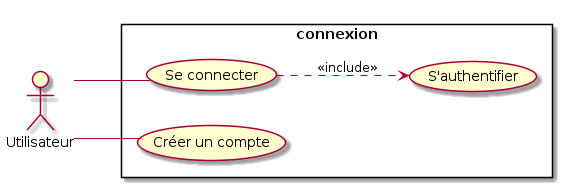
\includegraphics[width=0.9\textwidth]{../../res/uml/usecase/ConnexionUseCase.png}
    	\caption{Diagramme Use Case du Menu de Connexion}
    	\label{fig:main-menu}
\end{figure}
Le premier écran auquel l'utilisateur accède est un moyen de se connecter à la plateforme de jeu via un compte. Le moyen de s'authentifier est avec un compte existant et le mot de passe associé valide. Si l'utilisateur ne possède pas de compte existant, il peut en créer un nouveau avec un pseudo non existant sur la plateforme.


\subsubsection*{Connexion}
\begin{itemize}
    \item \textbf{Acteur}: Utilisateur
    \item \textbf{Use case}: Se connecter
    \item \textbf{Description}: Permet à l'utilisateur de se connecter au système.
    \item \textbf{Précondition}: L'utilisateur possède déjà un compte.
    \item \textbf{Postcondition}: L'utilisateur est connecté au système.
    \item \textbf{Cas exceptionnels}: Mauvais identifiant ou mot de passe, échec de la connexion réseau.
\end{itemize}

\subsubsection*{Créer un compte}
\begin{itemize}
    \item \textbf{Acteur}: Utilisateur
    \item \textbf{Use case}: Créer un compte
    \item \textbf{Description}: Permet à un utilisateur de s’inscrire et de se créer un compte.
    \item \textbf{Précondition}: L’utilisateur n’a pas encore de compte.
    \item \textbf{Postcondition}: Un nouveau compte est créé et l'utilisateur est authentifié.
    \item \textbf{Cas exceptionnels}: L'utilisateur existe déjà, erreurs de validation de données.
\end{itemize}

\subsubsection*{S'authentifier}
\begin{itemize}
    \item \textbf{Acteur}: Utilisateur
    \item \textbf{Use case}: S'authentifier
    \item \textbf{Description}: Vérifie les informations d'identification fournies par l'utilisateur.
    \item \textbf{Précondition}: L'utilisateur a soumis ses identifiants.
    \item \textbf{Postcondition}: Authentification réussie, session utilisateur créée.
    \item \textbf{Cas exceptionnels}: Identifiants incorrects, serveur d’authentification indisponible.
\end{itemize}

\newpage

\subsection{Menu Principal}

\begin{figure}[!h]
    \centering
    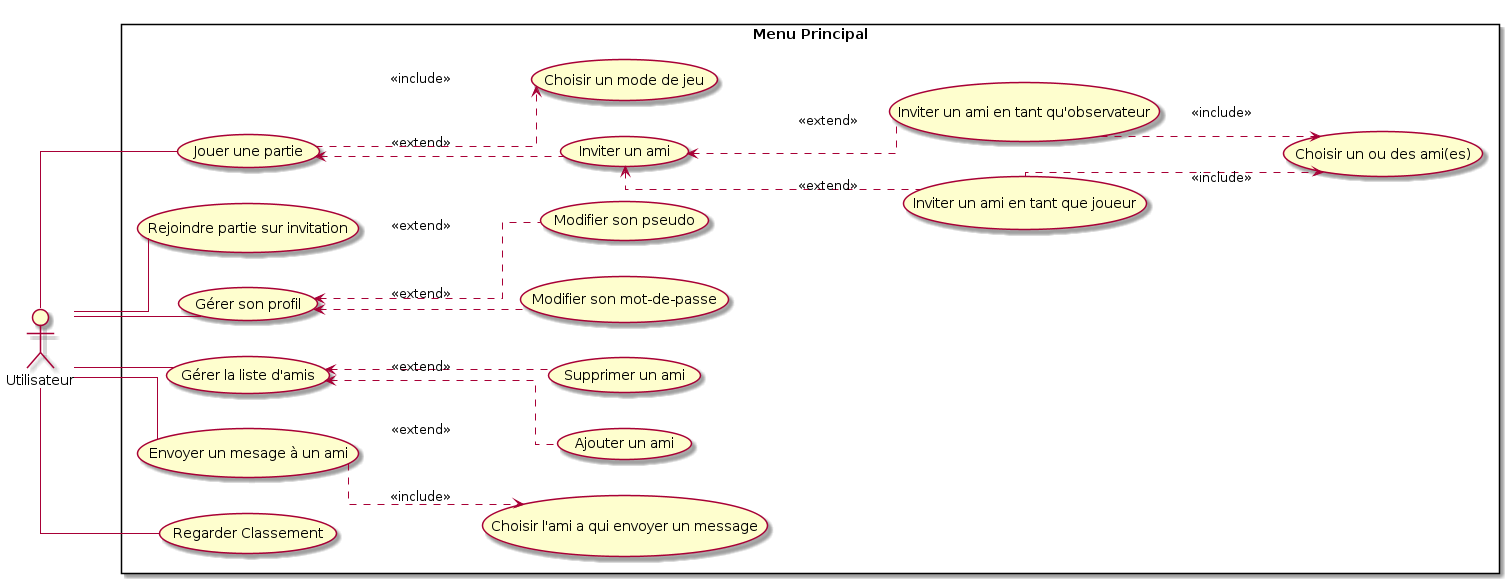
\includegraphics[width=1\textwidth]{../../res/uml/usecase/MenuPrincipalUseCase.png}
    \caption{Diagramme Use Case du Menu Principal}
    \label{fig:main-menu}
\end{figure}

Une fois l'authentification validée, l'écran du menu principal est accessible. L'utilisateur peut lancer une partie, gérer son profil, communiquer avec ses amis par la messagerie interne, gérer sa liste d'amis et regarder le classement général du jeu.

\subsubsection*{Jouer une partie}
\begin{itemize}
    \item \textbf{Acteur}: Utilisateur
    \item \textbf{Use case}: Jouer une partie
    \item \textbf{Description}: Permet à l'utilisateur de lancer une partie.
    \item \textbf{Précondition}: L'utilisateur est authentifié.
    \item \textbf{Postcondition}: Une partie de jeu est démarrée.
    \item \textbf{Cas exceptionnels}: Problème de connexion ou erreurs de lancement.
\end{itemize}

\subsubsection*{Rejoindre une partie existante}
\begin{itemize}
    \item \textbf{Acteur}: Utilisateur
    \item \textbf{Use case}: Rejoindre partie existante
    \item \textbf{Description}: Permet à l'utilisateur de rejoindre une partie existante sur invitation d'un ami.
    \item \textbf{Précondition}: L'utilisateur a reçu une invitation.
    \item \textbf{Postcondition}: L'utilisateur rejoint la partie.
    \item \textbf{Cas exceptionnels}: Invitation expirée ou la partie a atteint le nombre maximum de personnes.
\end{itemize}

\subsubsection*{Choisir mode de jeu}
\begin{itemize}
    \item \textbf{Acteur}: Utilisateur
    \item \textbf{Use case}: Choisir mode de jeu
    \item \textbf{Description}: Permet à l'utilisateur de choisir le mode de jeu.
    \item \textbf{Précondition}: L'utilisateur veut créer une partie de jeu.
    \item \textbf{Postcondition}: Le mode de jeu est défini pour la partie.
    \item \textbf{Cas exceptionnels}: Aucun.
\end{itemize}

\subsubsection*{Inviter un ami}
\begin{itemize}
    \item \textbf{Acteur}: Utilisateur
    \item \textbf{Use case}: Inviter un ami
    \item \textbf{Description}: Permet à l'utilisateur d'inviter un de ses amis présents dans sa liste à une partie.
    \item \textbf{Précondition}: L'ami est connecté.
    \item \textbf{Postcondition}: L'invitation est envoyée à l'ami.
    \item \textbf{Cas exceptionnels}: L'ami est indisponible ou décline l'invitation.
\end{itemize}

\subsubsection*{Gérer son profil}
\begin{itemize}
    \item \textbf{Acteur}: Utilisateur
    \item \textbf{Use case}: Gérer son profil
    \item \textbf{Description}: Permet à l'utilisateur de modifier les informations de son profil.
    \item \textbf{Précondition}: L'utilisateur est authentifié.
    \item \textbf{Postcondition}: Les informations de profil sont mises à jour.
    \item \textbf{Cas exceptionnels}: Échec de la mise à jour des informations.
\end{itemize}

\subsubsection*{Gérer la liste d'amis}
\begin{itemize}
    \item \textbf{Acteur}: Utilisateur
    \item \textbf{Use case}: Gérer la liste d'amis
    \item \textbf{Description}: Permet à l'utilisateur de gérer sa liste d'amis.
    \item \textbf{Précondition}: L'utilisateur est connecté.
    \item \textbf{Postcondition}: La liste d'amis est mise à jour.
    \item \textbf{Cas exceptionnels}: Problèmes de synchronisation, ami introuvable.
\end{itemize}

\subsubsection*{Envoyer un message à un ami}
\begin{itemize}
    \item \textbf{Acteur}: Utilisateur
    \item \textbf{Use case}: Envoyer un message à un ami
    \item \textbf{Description}: Permet à l'utilisateur d'envoyer un message à un ami.
    \item \textbf{Précondition}: L'ami est dans la liste d'amis.
    \item \textbf{Postcondition}: Le message est envoyé avec succès.
    \item \textbf{Cas exceptionnels}: Ami déconnecté ou problème de réseau.
\end{itemize}

\subsubsection*{Modifier son mot de passe}
\begin{itemize}
    \item \textbf{Acteur}: Utilisateur
    \item \textbf{Use case}: Modifier son mot de passe
    \item \textbf{Description}: Permet à l'utilisateur de changer son mot de passe.
    \item \textbf{Précondition}: L'utilisateur est authentifié.
    \item \textbf{Postcondition}: Le mot de passe est modifié avec succès.
    \item \textbf{Cas exceptionnels}: Mot de passe actuel incorrect, validation échouée.
\end{itemize}

\subsubsection*{Modifier son pseudo}
\begin{itemize}
    \item \textbf{Acteur}: Utilisateur
    \item \textbf{Use case}: Modifier son pseudo
    \item \textbf{Description}: Permet à l'utilisateur de changer son pseudo.
    \item \textbf{Précondition}: L'utilisateur est authentifié.
    \item \textbf{Postcondition}: Le pseudo est modifié avec succès.
    \item \textbf{Cas exceptionnels}: Le pseudo est déjà pris, le changement de pseudo est invalidé.
\end{itemize}

\subsubsection*{Ajouter un ami}
\begin{itemize}
    \item \textbf{Acteur}: Utilisateur
    \item \textbf{Use case}: Ajouter un ami
    \item \textbf{Description}: Permet à l'utilisateur d'ajouter un autre utilisateur à sa liste d'amis.
    \item \textbf{Précondition}: Le potentiel nouveau ami existe et est accessible.
    \item \textbf{Postcondition}: L'utilisateur est ajouté en tant qu'ami dans sa nouvelle liste.
    \item \textbf{Cas exceptionnels}: Ami déjà présent dans la liste ou utilisateur introuvable.
\end{itemize}

\subsubsection*{Supprimer un ami}
\begin{itemize}
    \item \textbf{Acteur}: Utilisateur
    \item \textbf{Use case}: Supprimer un ami
    \item \textbf{Description}: Permet à l'utilisateur de retirer un ami de sa liste.
    \item \textbf{Précondition}: L'ami existe dans la liste d'amis.
    \item \textbf{Postcondition}: L'ami est supprimé de la liste.
    \item \textbf{Cas exceptionnels}: L'utilisateur à supprimer n'est pas dans la liste d'amis.
\end{itemize}

\subsubsection*{Inviter un ami en tant que joueur}
\begin{itemize}
    \item \textbf{Acteur}: Utilisateur
    \item \textbf{Use case}: Inviter un ami en tant que joueur
    \item \textbf{Description}: L'utilisateur a créé une partie et invite un joueur dans sa liste d'amis dans la partie.
    \item \textbf{Précondition}: L'ami est connecté.
    \item \textbf{Postcondition}: Invitation envoyée pour jouer.
    \item \textbf{Cas exceptionnels}: L'ami n'est pas disponible et l'invitation est rejetée.
\end{itemize}

\subsubsection*{Inviter un ami en tant qu'observateur}
\begin{itemize}
    \item \textbf{Acteur}: Utilisateur
    \item \textbf{Use case}: Inviter un ami en tant qu'observateur
    \item \textbf{Description}: L'utilisateur a créé une partie et invite un ami de sa liste d'amis à la partie en tant qu'observateur.
    \item \textbf{Précondition}: L'ami est connecté.
    \item \textbf{Postcondition}: Invitation envoyée pour observer.
    \item \textbf{Cas exceptionnels}: L'ami est indisponible et l'invitation est rejetée.
\end{itemize}

\subsubsection*{Regarder Classement}
\begin{itemize}
    \item \textbf{Acteur}: Utilisateur
    \item \textbf{Use case}: Regarder Classement
    \item \textbf{Description}: Permet à l'utilisateur de consulter les classements.
    \item \textbf{Précondition}: L'utilisateur est connecté.
    \item \textbf{Postcondition}: Le classement est affiché.
    \item \textbf{Cas exceptionnels}: Classement indisponible, problèmes de connexion.
\end{itemize}

\newpage

\subsection{Différents modes de jeux}

\subsubsection{En mode Endless}

\begin{figure}[!h]
    \centering
    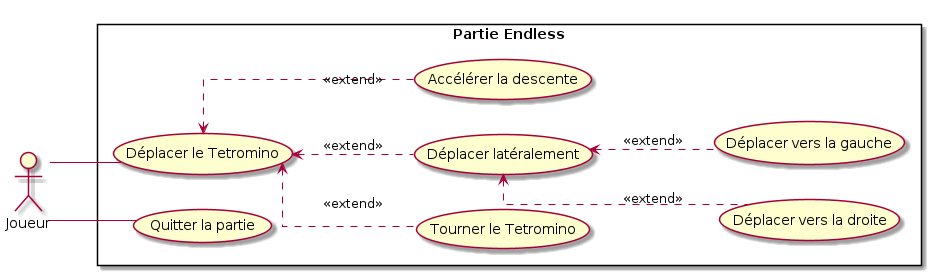
\includegraphics[width=1\textwidth]{../../res/uml/usecase/EndlessUseCase.png}
    \caption{Diagramme Use Case en mode Endless}
    \label{fig:Classique}
\end{figure}

\subsubsection*{Déplacer le Tetromino}
\begin{itemize}
    \item \textbf{Acteur}: Joueur
    \item \textbf{Use case}: Déplacer un Tetromino
    \item \textbf{Description}: Permet au joueur de déplacer un Tetromino sur le plateau.
    \item \textbf{Précondition}: Une partie est en cours et le joueur contrôle un Tetromino.
    \item \textbf{Postcondition}: Le Tetromino est déplacée dans une direction choisie.
    \item \textbf{Cas exceptionnels}: Limite du plateau atteinte, collision avec d'autres Tetromino.
\end{itemize}

\subsubsection*{Tourner le Tetromino}
\begin{itemize}
    \item \textbf{Acteur}: Joueur
    \item \textbf{Use case}: Tourner le Tetromino
    \item \textbf{Description}: Permet au joueur de tourner le Tetromino dans une direction donnée.
    \item \textbf{Précondition}: Une partie est en cours et un Tetromino est actif.
    \item \textbf{Postcondition}: Le Tetromino est tournée en conséquence.
    \item \textbf{Cas exceptionnels}: La rotation amène le Tetromino en dehors des limites.
\end{itemize}

% \subsubsection*{Menu pause}
% \begin{itemize}
%     \item \textbf{Acteur}: Joueur
%     \item \textbf{Use case}: Menu pause
%     \item \textbf{Description}: Permet au joueur d'ouvrir le menu de pause.
%     \item \textbf{Précondition}: La partie est en cours.
%     \item \textbf{Postcondition}: La partie est en pause.
%     \item \textbf{Cas exceptionnels}: Aucun.
% \end{itemize}

% \subsubsection*{Reprendre la partie}
% \begin{itemize}
%     \item \textbf{Acteur}: Joueur
%     \item \textbf{Use case}: Reprendre la partie
%     \item \textbf{Description}: Permet de reprendre la partie après une pause.
%     \item \textbf{Précondition}: La partie est en pause.
%     \item \textbf{Postcondition}: La partie reprend là où elle s'était arrêtée.
%     \item \textbf{Cas exceptionnels}: Aucun.
% \end{itemize}

\subsubsection*{Quitter la partie}
\begin{itemize}
    \item \textbf{Acteur}: Joueur
    \item \textbf{Use case}: Quitter la partie
    \item \textbf{Description}: Permet au joueur de quitter la partie en cours.
    \item \textbf{Précondition}: La partie est en cours.
    \item \textbf{Postcondition}: Le joueur quitte la partie et retourne au menu principal.
    \item \textbf{Cas exceptionnels}: Aucun.
\end{itemize}

\subsubsection{En mode Duel}

\begin{figure}[!h]
    \centering
    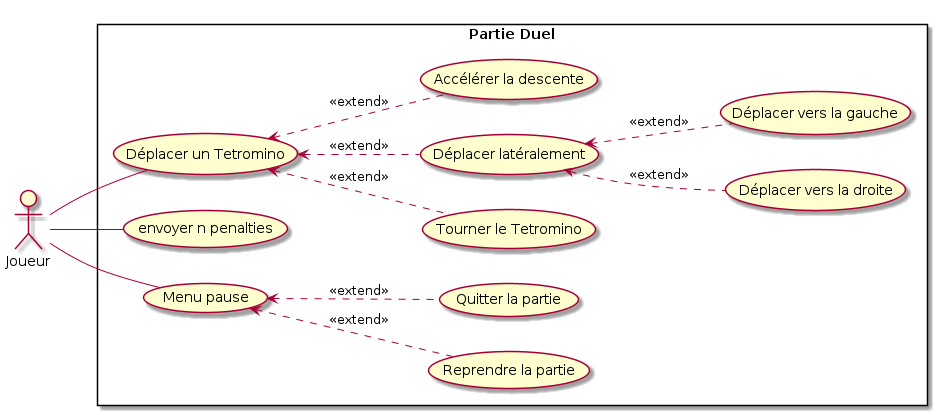
\includegraphics[width=1\textwidth]{../../res/uml/usecase/DualUseCase.png}
    \caption{Diagramme Use Case en mode Duel}
    \label{fig:Duel}
\end{figure}

\subsubsection*{Déplacer le Tetromino} (identique au mode Endless)

\subsubsection*{Tourner le Tetromino} (identique au mode Endless)

\subsubsection*{Envoyer n penalties}
\begin{itemize}
    \item \textbf{Acteur}: Joueur
    \item \textbf{Use case}: Envoyer n penalties
    \item \textbf{Description}: Envoie un ou plusieurs penalties à l'adversaire.
    \item \textbf{Précondition}: Le joueur a complété au moins deux lignes dans sa grille.
    \item \textbf{Postcondition}: L'adversaire reçoit un ou plusieurs penalties.
    \item \textbf{Cas exceptionnels}: Échec de l’envoi du penalty, conditions du penalty non remplies.
\end{itemize}

% \subsubsection*{Menu pause}
% \begin{itemize}
%     \item \textbf{Acteur}: Joueur
%     \item \textbf{Use case}: Menu pause
%     \item \textbf{Description}: Permet au joueur d'ouvrir le menu de pause.
%     \item \textbf{Précondition}: La partie est en cours.
%     \item \textbf{Postcondition}: La partie est en pause.
%     \item \textbf{Cas exceptionnels}: Aucun.
% \end{itemize}

% \subsubsection*{Reprendre la partie}
% \begin{itemize}
%     \item \textbf{Acteur}: Joueur
%     \item \textbf{Use case}: Reprendre la partie
%     \item \textbf{Description}: Permet de reprendre la partie après une pause.
%     \item \textbf{Précondition}: La partie est en pause.
%     \item \textbf{Postcondition}: La partie reprend là où elle s'était arrêtée.
%     \item \textbf{Cas exceptionnels}: Aucun.
% \end{itemize}

\subsubsection*{Quitter la partie}
\begin{itemize}
    \item \textbf{Acteur}: Joueur
    \item \textbf{Use case}: Quitter la partie
    \item \textbf{Description}: Permet au joueur de quitter la partie en cours.
    \item \textbf{Précondition}: La partie est en cours.
    \item \textbf{Postcondition}: Le joueur quitte la partie et retourne au menu principal.
    \item \textbf{Cas exceptionnels}: Aucun.
\end{itemize}

\subsubsection{En mode Classique}

\begin{figure}[!h]
    \centering
    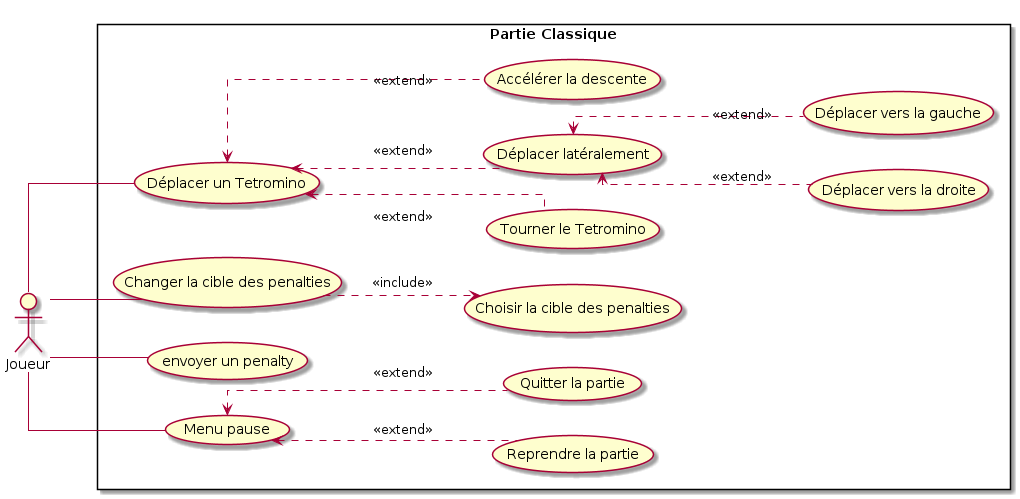
\includegraphics[width=1\textwidth]{../../res/uml/usecase/ClassicUseCase.png}
    \caption{Diagramme Use Case en mode Classique}
    \label{fig:Endless}
\end{figure}

\subsubsection*{Déplacer le Tetromino} (identique au mode Endless)
\subsubsection*{Tourner le Tetromino} (identique au mode Endless)
\subsubsection*{Accélérer la descente} (identique au mode Endless)
\subsubsection*{Déplacer latéralement} (identique au mode Endless)

\subsubsection*{Changer la cible des penalties}
\begin{itemize}
    \item \textbf{Acteur}: Joueur
    \item \textbf{Use case}: Changer la cible des penalties
    \item \textbf{Description}: Permet au joueur de changer l'adversaire recevant le penalty
    \item \textbf{Précondition}: La partie est en cours et le joueur peut envoyer un ou plusieurs penalties.
    \item \textbf{Postcondition}: Le joueur a sélectionné une nouvelle cible pour envoyer ses penalties.
    \item \textbf{Cas exceptionnels}: Il n'y a plus d'autres joueurs dans la partie.
\end{itemize}

\subsubsection*{Choisir la cible des penalties}
\begin{itemize}
    \item \textbf{Acteur}: Joueur
    \item \textbf{Use case}: Choisir la cible des penalties
    \item \textbf{Description}: Le joueur choisit parmis ses adversaires sa nouvelle cible pour les penalties.
    \item \textbf{Précondition}: La partie est en cours et le joueur peut envoyer un penalty.
    \item \textbf{Postcondition}: Le joueur change de cible et envoie un ou plusieurs penalties à l’adversaire nouvellement désigné.
    \item \textbf{Cas exceptionnels}: Il n'y a plus d'autres joueurs dans la partie.
\end{itemize}

\subsubsection*{Envoyer n penalties} (identique au mode Duel)

% \subsubsection*{Menu pause} (identique au mode Duel)
% \subsubsection*{Reprendre la partie} (identique au mode Duel)
\subsubsection*{Quitter la partie} (identique au mode Duel)

\subsubsection{En mode Royal Competition}

\begin{figure}[!h]
    \centering
    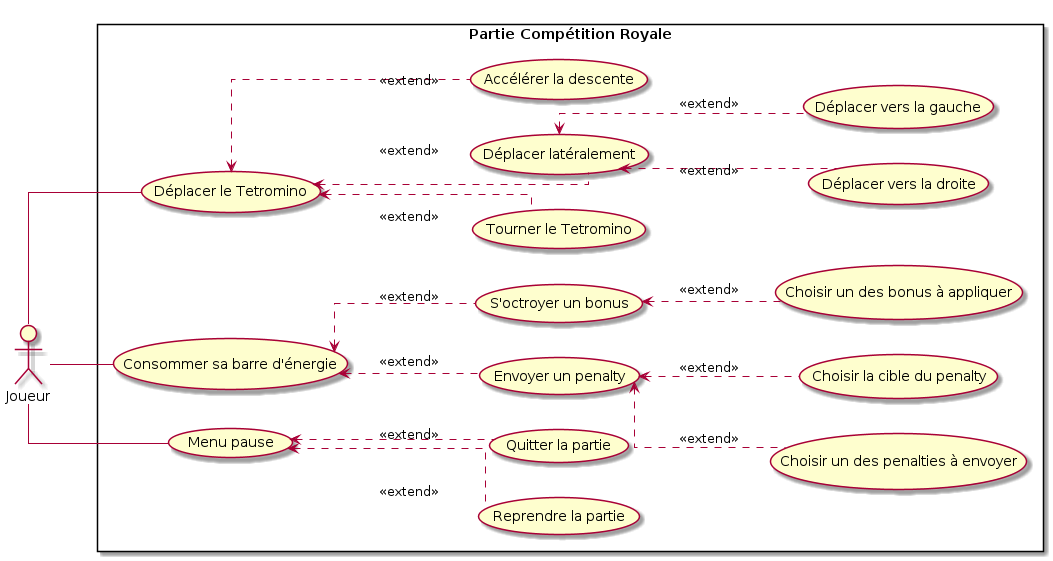
\includegraphics[width=1\textwidth]{../../res/uml/usecase/RoyalUseCase.png}
    \caption{Diagramme Use Case en mode Royal Competition}
    \label{fig:Royal-Competition}
\end{figure}

\subsubsection*{Déplacer le Tetromino} (identique au mode Endless)
\subsubsection*{Tourner le Tetromino} (identique au mode Endless)
\subsubsection*{Déplacer latéralement} (identique au mode Endless)
\subsubsection*{Accélérer la descente} (identique au mode Endless)

\subsubsection*{Consommer sa barre d'énergie}
\begin{itemize}
    \item \textbf{Acteur}: Joueur
    \item \textbf{Use case}: Consommer sa barre d'énergie
    \item \textbf{Description}: Le joueur a accumulé assez d'énergie dans sa barre avec des lignes complétées dans sa grille et consomme une partie de son énergie.
    \item \textbf{Précondition}: La partie est en cours et le joueur a accumulé assez de lignes complétées.
    \item \textbf{Postcondition}: Le joueur consomme sa barre d'énergie parmis les différents actions proposées.
    \item \textbf{Cas exceptionnels}: Il n'y a plus d'autres joueurs dans la partie.
\end{itemize}

\subsubsection*{S'octroyer un bonus}
\begin{itemize}
    \item \textbf{Acteur}: Joueur
    \item \textbf{Use case}: S'octroyer un bonus
    \item \textbf{Description}: Le joueur applique un bonus sur son jeu.
    \item \textbf{Précondition}: La partie est en cours et le joueur peut consommer sa barre d'énergie.
    \item \textbf{Postcondition}: Le joueur reçoit le bonus applicable durant un temps donné. 
    \item \textbf{Cas exceptionnels}: Il n'y a plus d'autres joueurs dans la partie.
\end{itemize}

\subsubsection*{Envoyer un penalty}
\begin{itemize}
    \item \textbf{Acteur}: Joueur
    \item \textbf{Use case}: Envoyer un penalty
    \item \textbf{Description}: Le joueur envoie un penalty à l'adversaire choisi.
    \item \textbf{Précondition}: La partie est en cours et le joueur peut envoyer un penalty à un adversaire.
    \item \textbf{Postcondition}: Le joueur envoie le penalty à l'adversaire choisi.
    \item \textbf{Cas exceptionnels}: Il n'y a plus d'autres joueurs dans la partie. 
\end{itemize}

\subsubsection*{Choisir un des penalties à envoyer}
\begin{itemize}
    \item \textbf{Acteur}: Joueur
    \item \textbf{Use case}: choisir un des penalties à envoyer
    \item \textbf{Description}: Le joueur a plusieurs options de penalties à envoyer à l'adversaire choisi.
    \item \textbf{Précondition}: La partie est en cours et le joueur peut consommer sa barre d'énergie.
    \item \textbf{Postcondition}: Le joueur envoie un des penalties proposés à l'adversaire visé.
    \item \textbf{Cas exceptionnels}: Il n'y a plus d'autres joueurs dans la partie.
\end{itemize}

\subsubsection*{Choisir la cible du penalties} (identique au mode Classique)
% \subsubsection*{Menu pause} (identique au mode Duel)
% \subsubsection*{Reprendre la partie} (identique au mode Duel)
\subsubsection*{Quitter la partie} (identique au mode Duel)

\newpage

\section{Besoin système : Fonctionnels}

\subsection{Connexion}

\quad Quand l'utilisateur ouvre l'application, il doit avoir un compte valide pour s'authentifier. Il doit fournir le nom du compte et le mot de passe.\\
Ses entrées sur les deux champs sont envoyées au serveur de l'application. Les données sont vérifiées en recherchant dans la base de données un profil correspondant. Si un compte est trouvé avec le mot de passe correctement entré, le serveur connecte l'utilisateur au compte associé. Mais s'il ne trouve pas dans la base de données, l'utilisateur est notifié d'un message d'erreur du serveur.

\subsection{Gestion des comptes}

\subsubsection{Création d'un compte}

Quand un utilisateur crée un compte, il doit fournir un nom de compte et un mot de passe. Chaque entrée saisie a une taille minimale, maximale et une restriction sur les caractères autorisés. Le nom utilisé doit être unique pour chaque compte.\\
Le serveur vérifie qu'il n'existe pas déjà une autre entrée possédant le même nom. 

\subsubsection{Suppression d'un compte}

L'option de suppression du compte doit être possible sur le système. Quand l'utilisateur fait une telle demande en confirmant avec son mot de passe associé, le programme client le questionne une dernière fois avant d'envoyer la requête au serveur. Le serveur supprime l'entrée sur la base de données du compte en question et l'utilisateur est déconnecté de la session.

\subsection{Consulter le classement}

Quand l'utilisateur est connecté et en dehors d'une partie de jeu, il peut consulter le classement général des joueurs de la plateforme pour le mode de jeu \textit{Endless}. Le serveur l'actualise à chaque fin de partie et l'envoie sous forme de requête à chaque utilisateur concernant le classement.

\subsection{Gestion de la partie}

De la création à la fin de la partie, toutes les actions de l'utilisateur sont envoyées sous forme de requête au serveur et ce dernier applique l'action si elle est possible (ex. placer une pièce à tel endroit de la grille, envoyer un penalty à un adversaire, etc.). Le serveur permet de valider les actions et de vérifier s'il n'y a pas de triche en cours. La partie modifiée par le serveur avec la nouvelle action intégrée ou non sera récupérée et affichée à l'utilisateur.

\subsection{Gestion des amis}

Quand un utilisateur veut rajouter un autre utilisateur existant sur la plateforme à sa liste d'amis, le programme client enverra une requête au serveur. Si cette entrée saisie se trouve dans la base de données de l'application, le serveur enverra une requête au programme client de l'autre utilisateur. Ce dernier recevra une requête d'une demande d'ami qu'il pourra accepter ou non.

\subsubsection{Gestion du chat}

L'utilisateur peut utiliser la messagerie interne de l'application quand il possède au minimum un ami dans sa liste. Quand un message est envoyé de l'utilisateur, il est envoyé sous forme de requête utilisateur au serveur. Le ou les destinataires du message sont transmis au programme client de ces derniers. L'opération s'effectue sous condition d'avoir une connexion stable au serveur.

\subsection{Fin de la partie}

\subsubsection{Fin de la partie \textit{Endless}}

Lorsque le joueur ne peut plus placer un \textit{tetromino} sur sa grille ou demande volontairement d'arrêter de jouer, la partie se termine. Le serveur modifie le meilleur score associé au compte de l'utilisateur s'il a battu son propre record. Le classement des joueurs de l'application est mis à jour s'il y a eu modifications. 

\subsubsection{Fin de la partie \textit{Multijoueurs}}

Dans une partie de \textit{Tetris} à plusieurs joueurs, le gagnant est celui qui peut toujours placer des \textit{tetrominoes} sur sa grille tandis que les autres joueurs n'ont plus d'espace pour en déposer un.

\section{Besoins système : Non fonctionnels}

\subsection{Besoins système}

\subsubsection{Réseau}

%Le jeu doit se jouer en réseau car il a besoin de se connecter au serveur.

L'application demande une connexion internet avec le protocole TCP/IP pour connecter le client au serveur. Ce n'est pas requis quand les deux se trouvent sur la même machine; cela n'est pas attendu dans le cadre d'utilisation de l'application.

\subsubsection{Système d'exploitation}

Les machines du client et du serveur doivent pouvoir s'exécuter sur un système d'exploitation \texttt{Linux}.

\subsubsection{Accessibilité}

Le client doit être connecté à internet pour accéder au serveur. Son utilisation est gratuite pour tout utilisateur qui s'authentifie à un compte valable. S'il n'en possède pas un existant, il peut facilement s'en créer un. 

\subsubsection{Performances}

%Les temps de rafraîchissement et les temps de réponses seront en millisecondes.

Afin de minimiser le nombre de requêtes du client au serveur, des conditions seront vérifiées par le client avant d'envoyer ces dernières au serveur. \\

\textit{Exemple} : l'utilisateur a bien fait au minimum deux combinaisons de lignes avant de pouvoir envoyer un ou plusieurs penalties à un de ses adversaires.

\subsubsection{Capacité}

%Le jeu pourra lancer une partie jusqu'à neuf joueurs pour le mode classique et acceptera aussi des spectateurs pour voir la partie en cours. L'espace de stockage sera quelques Megabytes.

Plusieurs parties de maximum neuf joueurs peuvent se tenir en même temps sur le serveur. De plus, l'espace de stockage pour chaque partie doit être au maximum de quelques mégaoctets.

\subsubsection{Sécurité}

%Pour accéder au jeu, l'utilisateur devra s'authentifier à l'aide d'un pseudo et un mot de passe.

Pour accéder au jeu, l'utilisateur devra s'authentifier à l'aide d'un nom d'utilisateur et de son mot de passe associé. Notamment, le serveur devra vérifier l'application correcte de toutes les règles du jeu durant la partie afin d'éviter des triches de la part des utilisateurs.

\subsubsection{Robustesse}

S'il reste au moins trois joueurs et que l'un d'entre eux se déconnecte de la partie ou du serveur, le jeu doit pouvoir continuer fluidement sans interruption. Celui qui vient de quitter la partie se retrouve perdant et est placé à la bonne position du classement de cette dernière.

\subsection{Besoins utilisateur}

L'application doit proposer une interface graphique intuitive à utiliser pour le joueur. Cela comprend un choix d'apparence attrayante en gardant une orientation d'une implémentation d'un jeu.\\
 De plus, pour permettre une meilleure expérience de l'application à l'utilisateur, le lancement d'une partie locale ou avec une connexion au serveur doit être fluide et stable. La même chose est attendue durant tout le jeu. Le temps de rafraîchissement de l'interface du client doit se faire dans l'ordre du dixième de seconde.

\newpage

\section{Architecture du système}

\subsection{Architecture du jeu}

\subsubsection{Classes du jeu}

Au lancement d'une partie sur l'application, chaque joueur possède un objet de la classe Tetris. Dans la Board et la \textit{queue-list} de tetrominoes, attributs de Tetris, le joueur placera les formes sur la Board. En reprenant l'algorithme pré-existant dans d'autres implémentations du jeu \textit{Tetris}, le tetromino effectue une rotation similaire au fonctionnement de \textit{Super Rotation System}. À chaque action du joueur envoyé pour changer la position du tetromino, Tetris calcule la nouvelle position selon celle renvoyée par le tetromino et puis vérifie la validité de cette position dans la Board. 

Au lancement d'une partie avec plusieurs joueurs ou non, pour chaque joueur, nous avons la création d'un objet Tetris et PlayerState réunis dans un PlayerTetris. Pour l'ensemble de la partie, nous aurons un objet GameState qui contient toutes les informations nécessaires pour connaitre la situation de la partie en cours. Puis l'objet GameEngine permettra de valider ou non les actions demandées par les joueurs (\textit{ex. changer le tetromino de rotation}).

\newpage

\begin{figure}[H]
	\centering
	 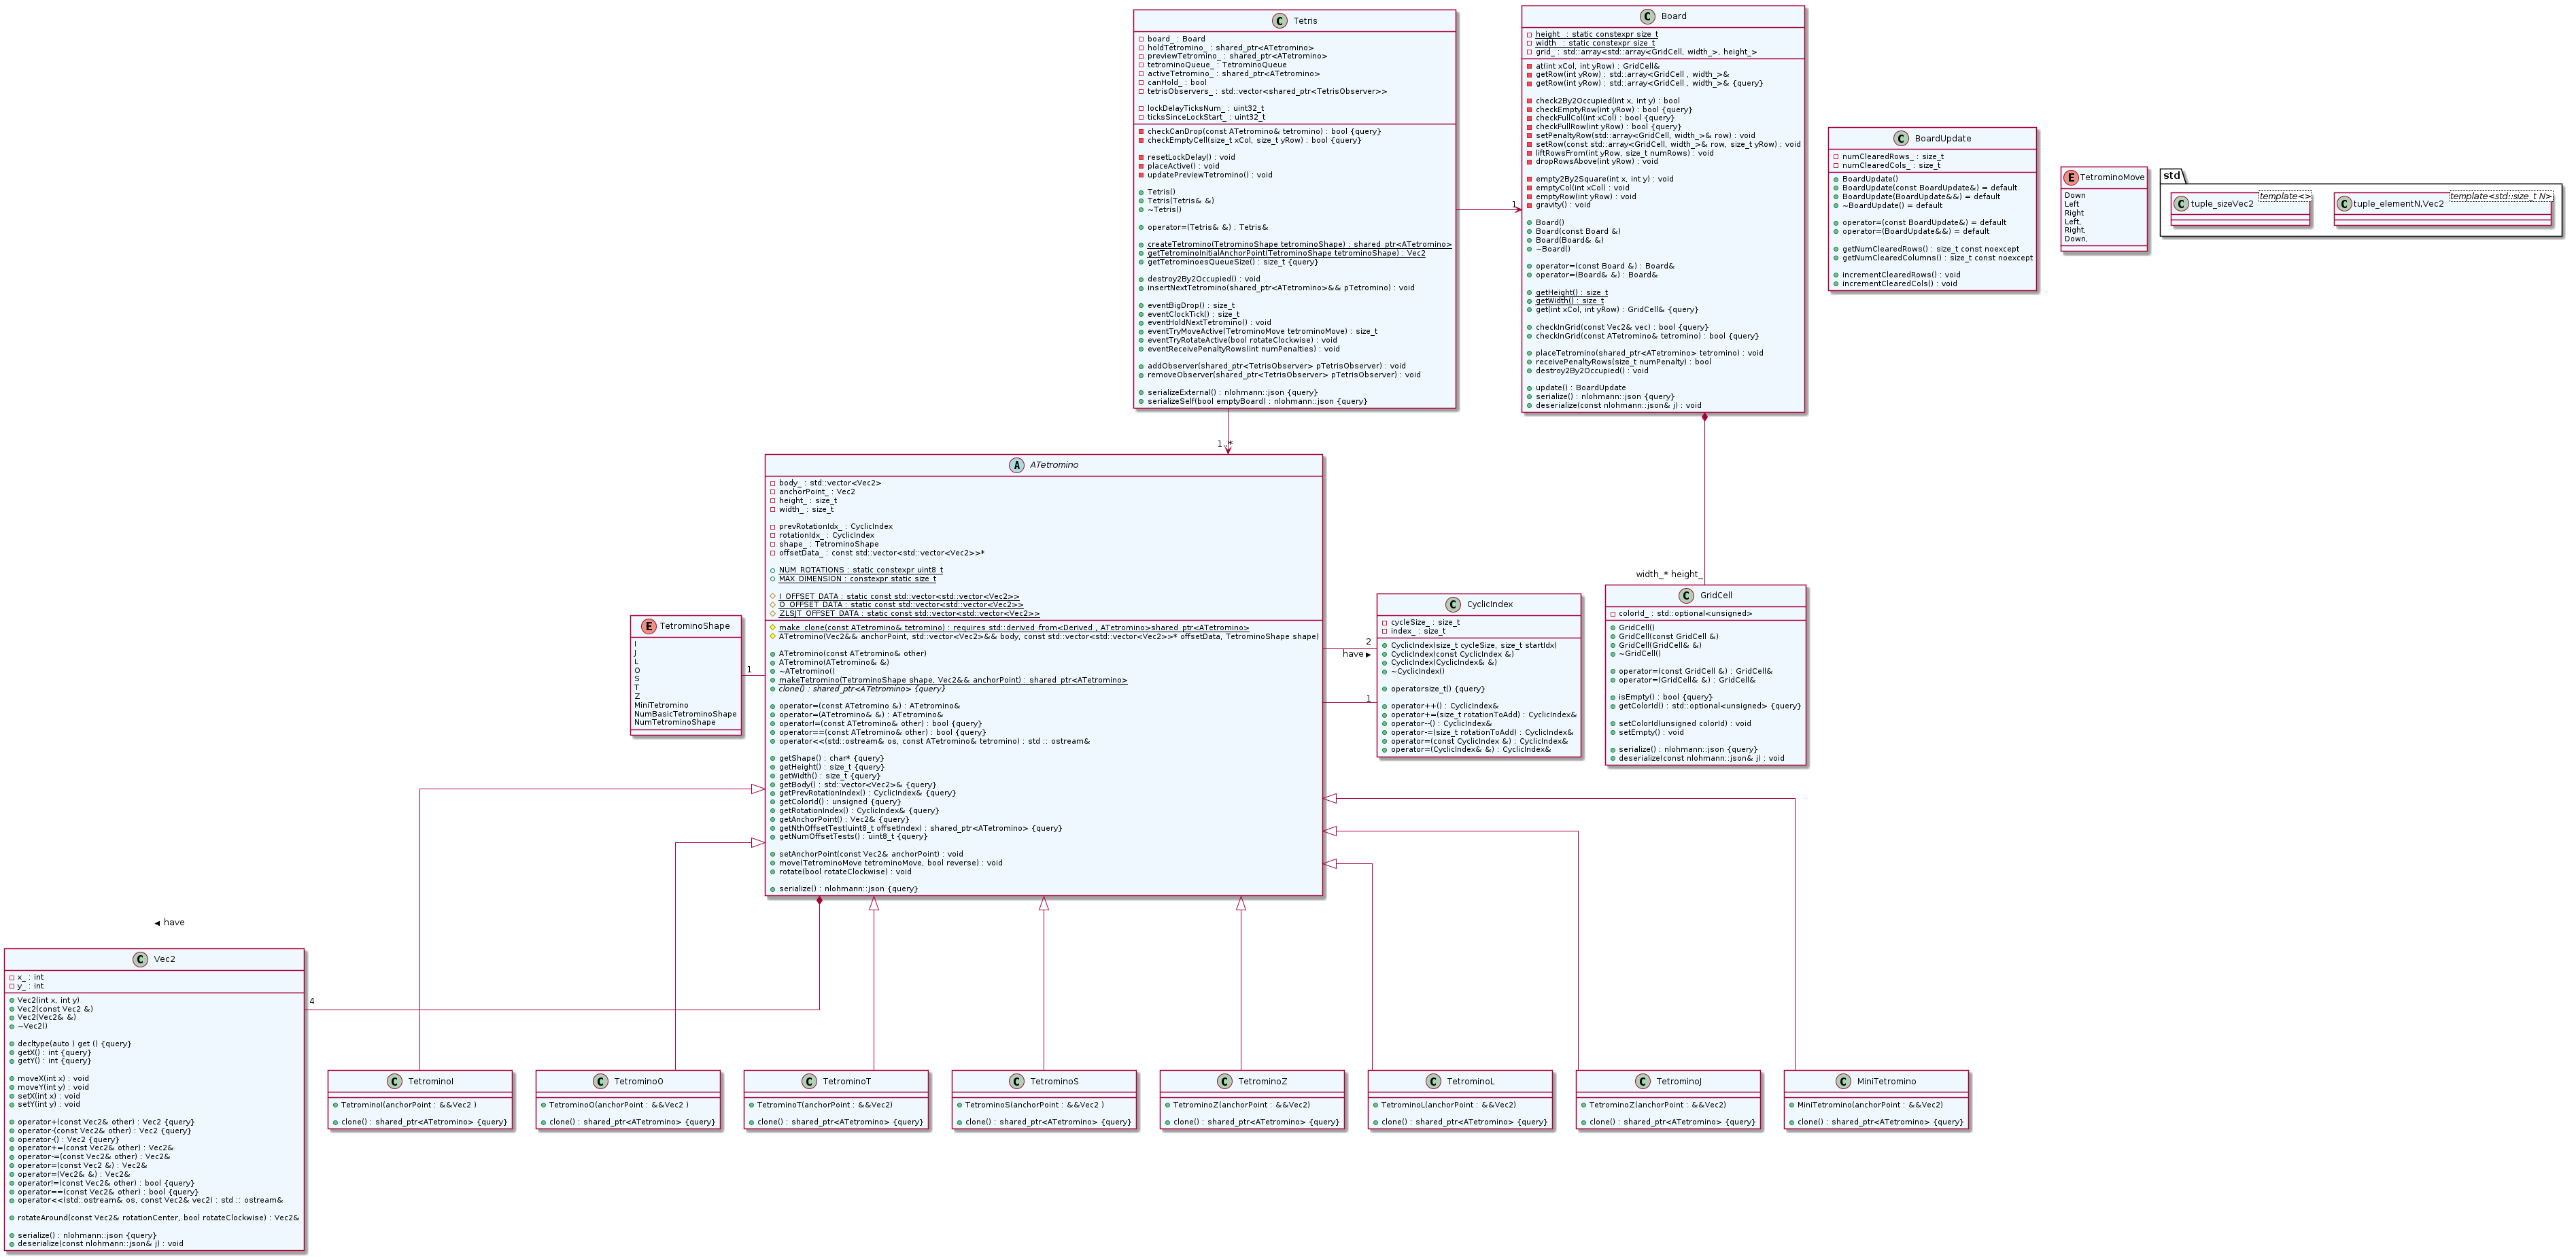
\includegraphics[scale=0.2, angle=90]{../../res/uml/class/GameClass.png}
	 \caption{Diagramme de classes de Game}
	 \label{fig:GameClassDiagram}
\end{figure}


\subsubsection*{PlayerState}

Le PlayerState permet d'associer le joueur, ses informations sur son avancemment durant la partie et celle de son profil.

\begin{figure}[!h]
	\centering
	 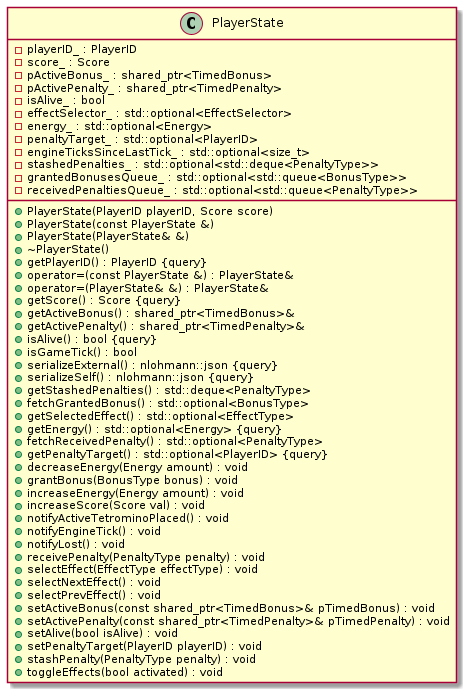
\includegraphics[scale=0.6]{../../res/uml/class/PlayerStateClass.png}
	 \caption{Diagramme de classe de PlayerState}
	 \label{fig:PlayerStateDiagram}
\end{figure}

\subsubsection*{PlayerTetris}

Le PlayerTetris permet d'associer un PlayerState et un Tetris.

\begin{figure}[!h]
	\centering
	 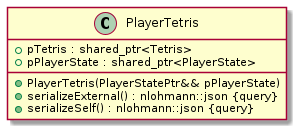
\includegraphics[scale=0.6]{../../res/uml/class/PlayerTetrisClass.png}
	 \caption{Diagramme de classe de PlayerTetris}
	 \label{fig:PlayerTetrisDiagram}
\end{figure}

\subsubsection*{GameState}

Le GameState permet d'associer à une partie multijoueur ou non, un vecteur de PlayerState selon le nombre de participants. Il permet également d'accéder à un PlayerState selon l'identifiant du joueur pour pouvoir appliquer des actions dessus.

\begin{figure}[!h]
	\centering
	 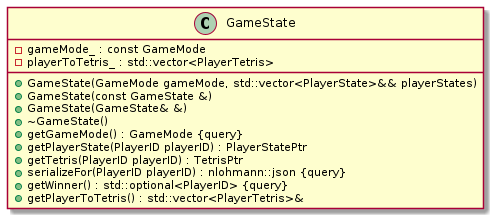
\includegraphics[scale=0.6]{../../res/uml/class/GameStateClass.png}
	 \caption{Diagramme de classe de GameState}
	 \label{fig:GameStateDiagram}
\end{figure}


\subsubsection*{GameEngine}

Le GameEngine permet de changer l'état de GameState selon les méthodes appélées pour faire des actions sur la grille d'un joueur de la partie (\textit{ex. changer la roation du tetromino active}) ou entre eux (\textit{ex. envoyer une pénalité à un adversaire}). 

\begin{figure}[H]
	\centering
	 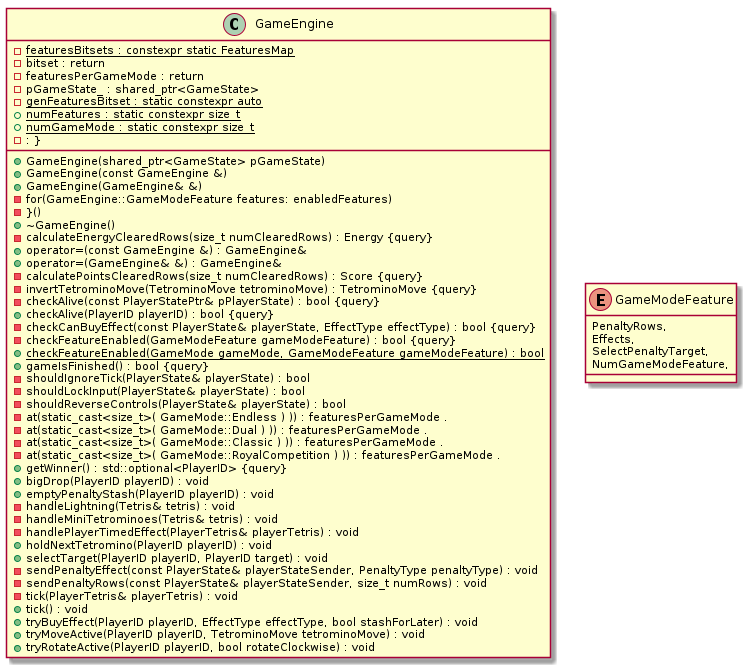
\includegraphics[scale=0.5]{../../res/uml/class/GameEngineClass.png}
	 \caption{Diagramme de classe de GameEngine}
	 \label{fig:GameEngine}
\end{figure}

\subsubsection{Partie multijoueur en mode royal}

Au lancement d'une partie mulitjoueur dans le mode royal, pour chaque joueur, nous avons la création d'un objet Tetris et PlayerState. Contrairement aux autres modes, le PlayerState contient des informations supplémentaires tel que le niveau de la barre d'énergie et une queue de penalités à venir sur le joueur en question. Pour l'ensemble de la partie, GameEngine permettra de valider les actions demandées par les joueurs comprenant également les conditions pour acheter un effect spécifique.
\subsubsection*{Les effects}

Pour l'implémentation des effects, nous avons distingué trois grandes familles, les effects qui s'écoulent sur une période de temps, les effects qui s'écoulent au bout d'un nombre de mouvements du joueur et les effects qui vont uniquement changer la grille d'un joueur une seule fois.

Nous avons une classe abstraite qui déclare des méthodes pour avoir le temps écoulé et le nombre de mouvements du joueur. Ces méthodes sont concrétisées dans l'implémentation de deux classes héritantes, une pour les nombres d'actions restantes avant que l'effet se termine et une autre pour la durée restante. Puis les effects sont séparés en deux catégories, des bonus ou des penalités regroupées dans leur enumération de type respective. 

\begin{figure}[H]
    \centering
    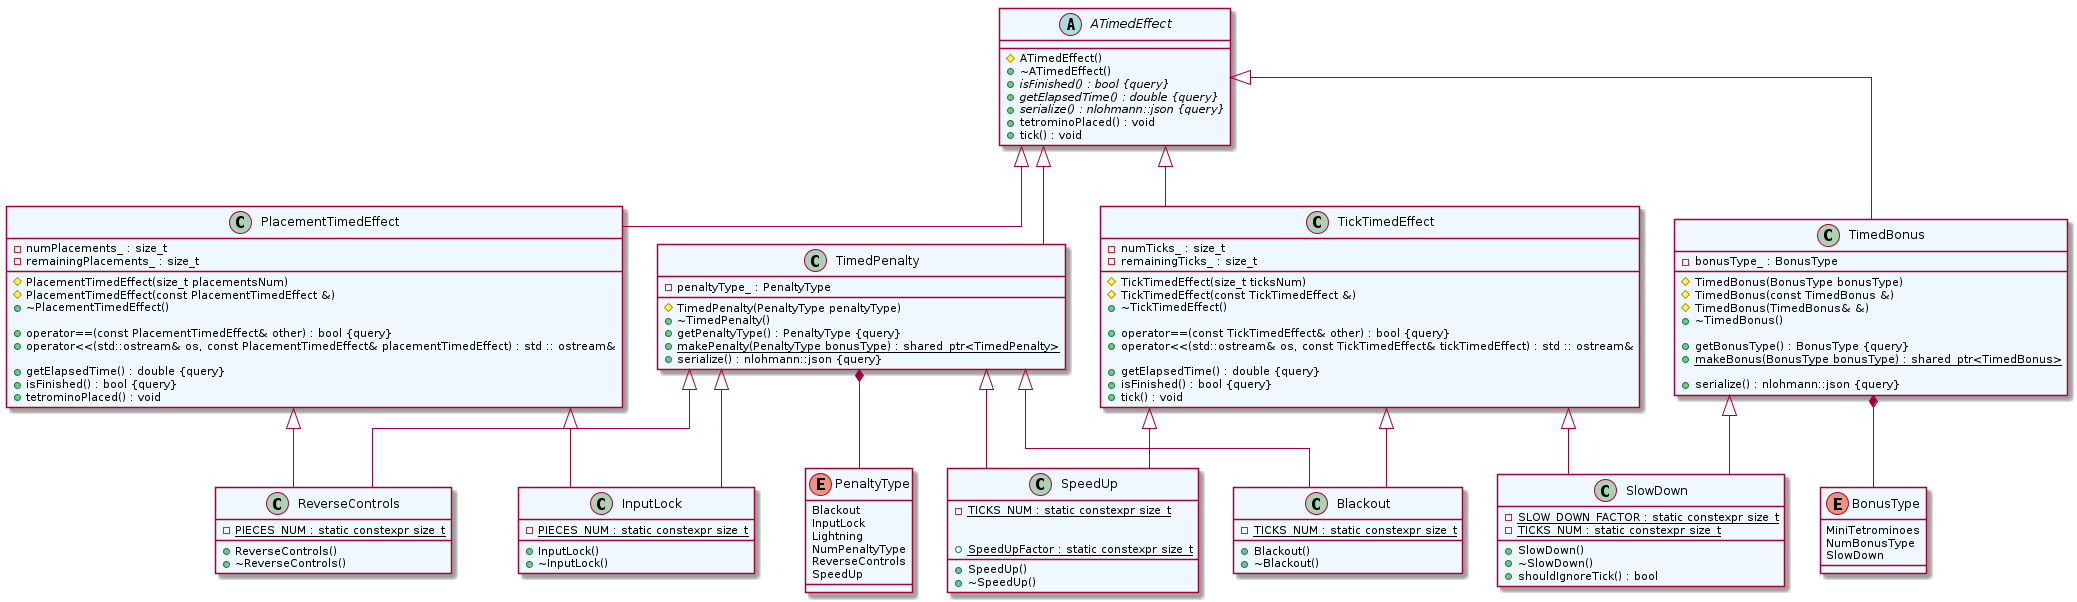
\includegraphics[scale=0.3, angle=90]{../../res/uml/class/EffectClass.png}
    \caption{Diagramme de classes des effects}
    \label{fig:EffectDiagramm}
\end{figure}

\subsubsection{Diagramme complet du jeu}

\begin{figure}[H]
    \centering
    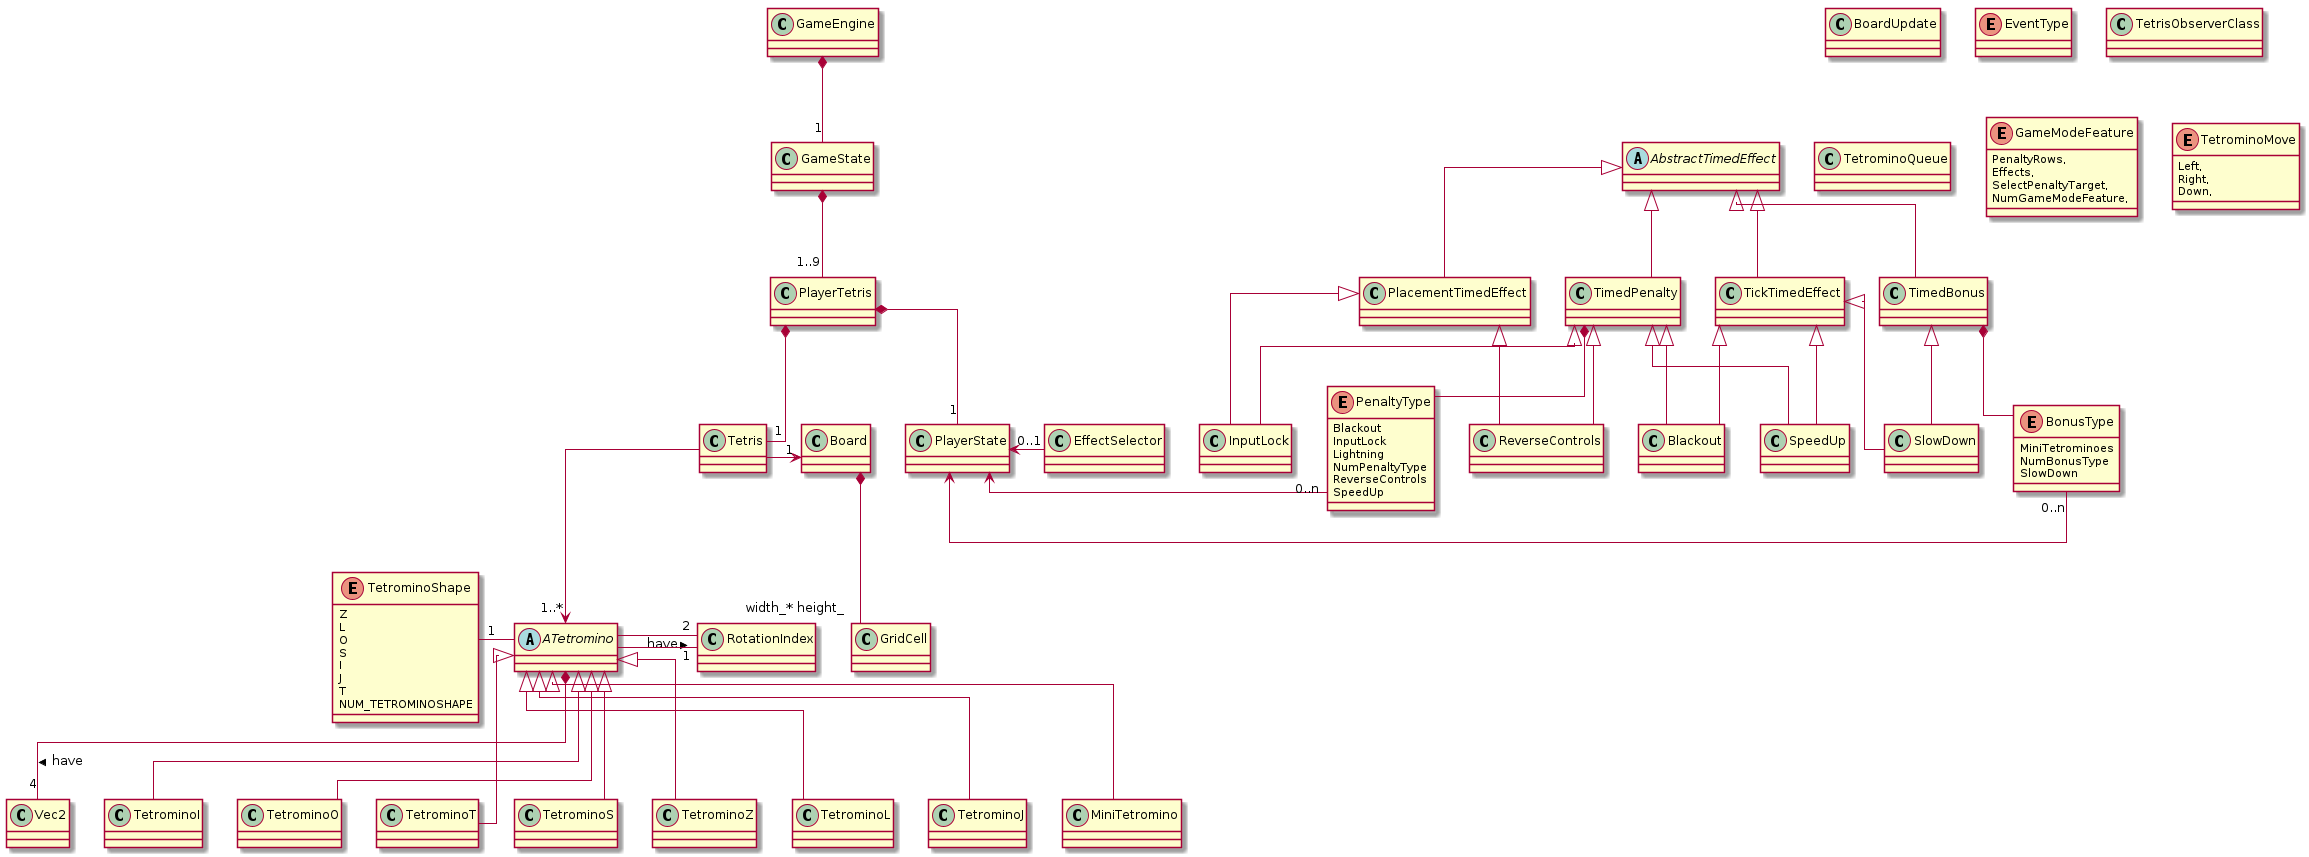
\includegraphics[scale=0.3, angle=90]{../../res/uml/class/GameStructureClass.png}
    \caption{Diagramme de classes simplifiées du jeu}
    \label{fig:WholeGameDiagramm}
\end{figure}

\newpage


\subsection{Architecture du serveur}

Le serveur est composé de quatre parties différentes. Chacune a un but précis pour permettre la communication entre différents utilisateurs.

\subsubsection{La base de données}

La base de données permet de stocker des informations sur les différents utilisateurs qui possèdent un compte dans l'application. Nous avons quatre différentes classes pour la base de données. 
\begin{itemize}
	\item AccountManager regroupe les informations du profil d'un utilisateur et permet de les modifier.
	\item FriendsManager permet de modifier ou de regarder la liste d'amis selon l'identifiant de l'utilisateur.
	\item MessagesManager gère le stockage de la messagerie de tous les utilisateurs et permet d'ajouter des messages à un fil de discussion existante ou qui va être créée sous certaines conditions. 
	\item DatabaseManager permet de faire des redirections de requêtes pour les objets extérieurs qui vont faire une demande indirecte de changement de contenu de la base de données.
\end{itemize}

\begin{figure}[!ht]
	\centering
	 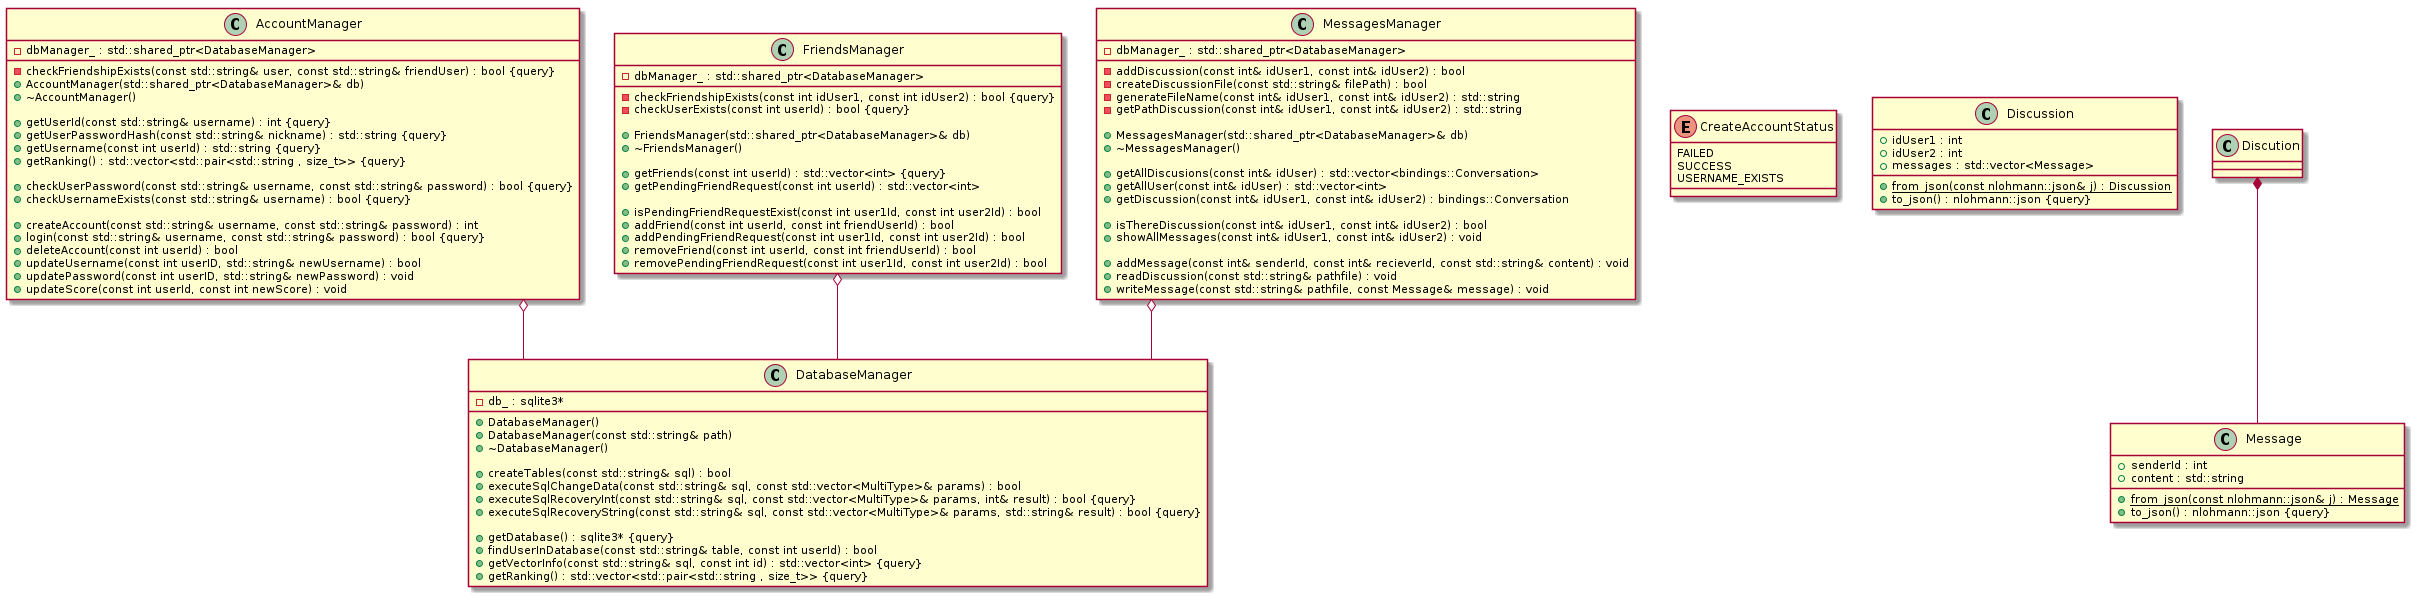
\includegraphics[scale=0.2]{../../res/uml/class/DatabaseClass.png}
	 \caption{Diagramme de classes de la base de données}
	 \label{fig:DatabaseDiagram}
\end{figure}

\subsubsection{Le network}

\subsubsection*{Les bindings}

Nous avons implémenté un espace de nommage \textit{bindings}. Cela permet d'avoir un standard sur les paquets que le serveur peut recevoir et envoyer.

\begin{figure}[H]
	\centering
	 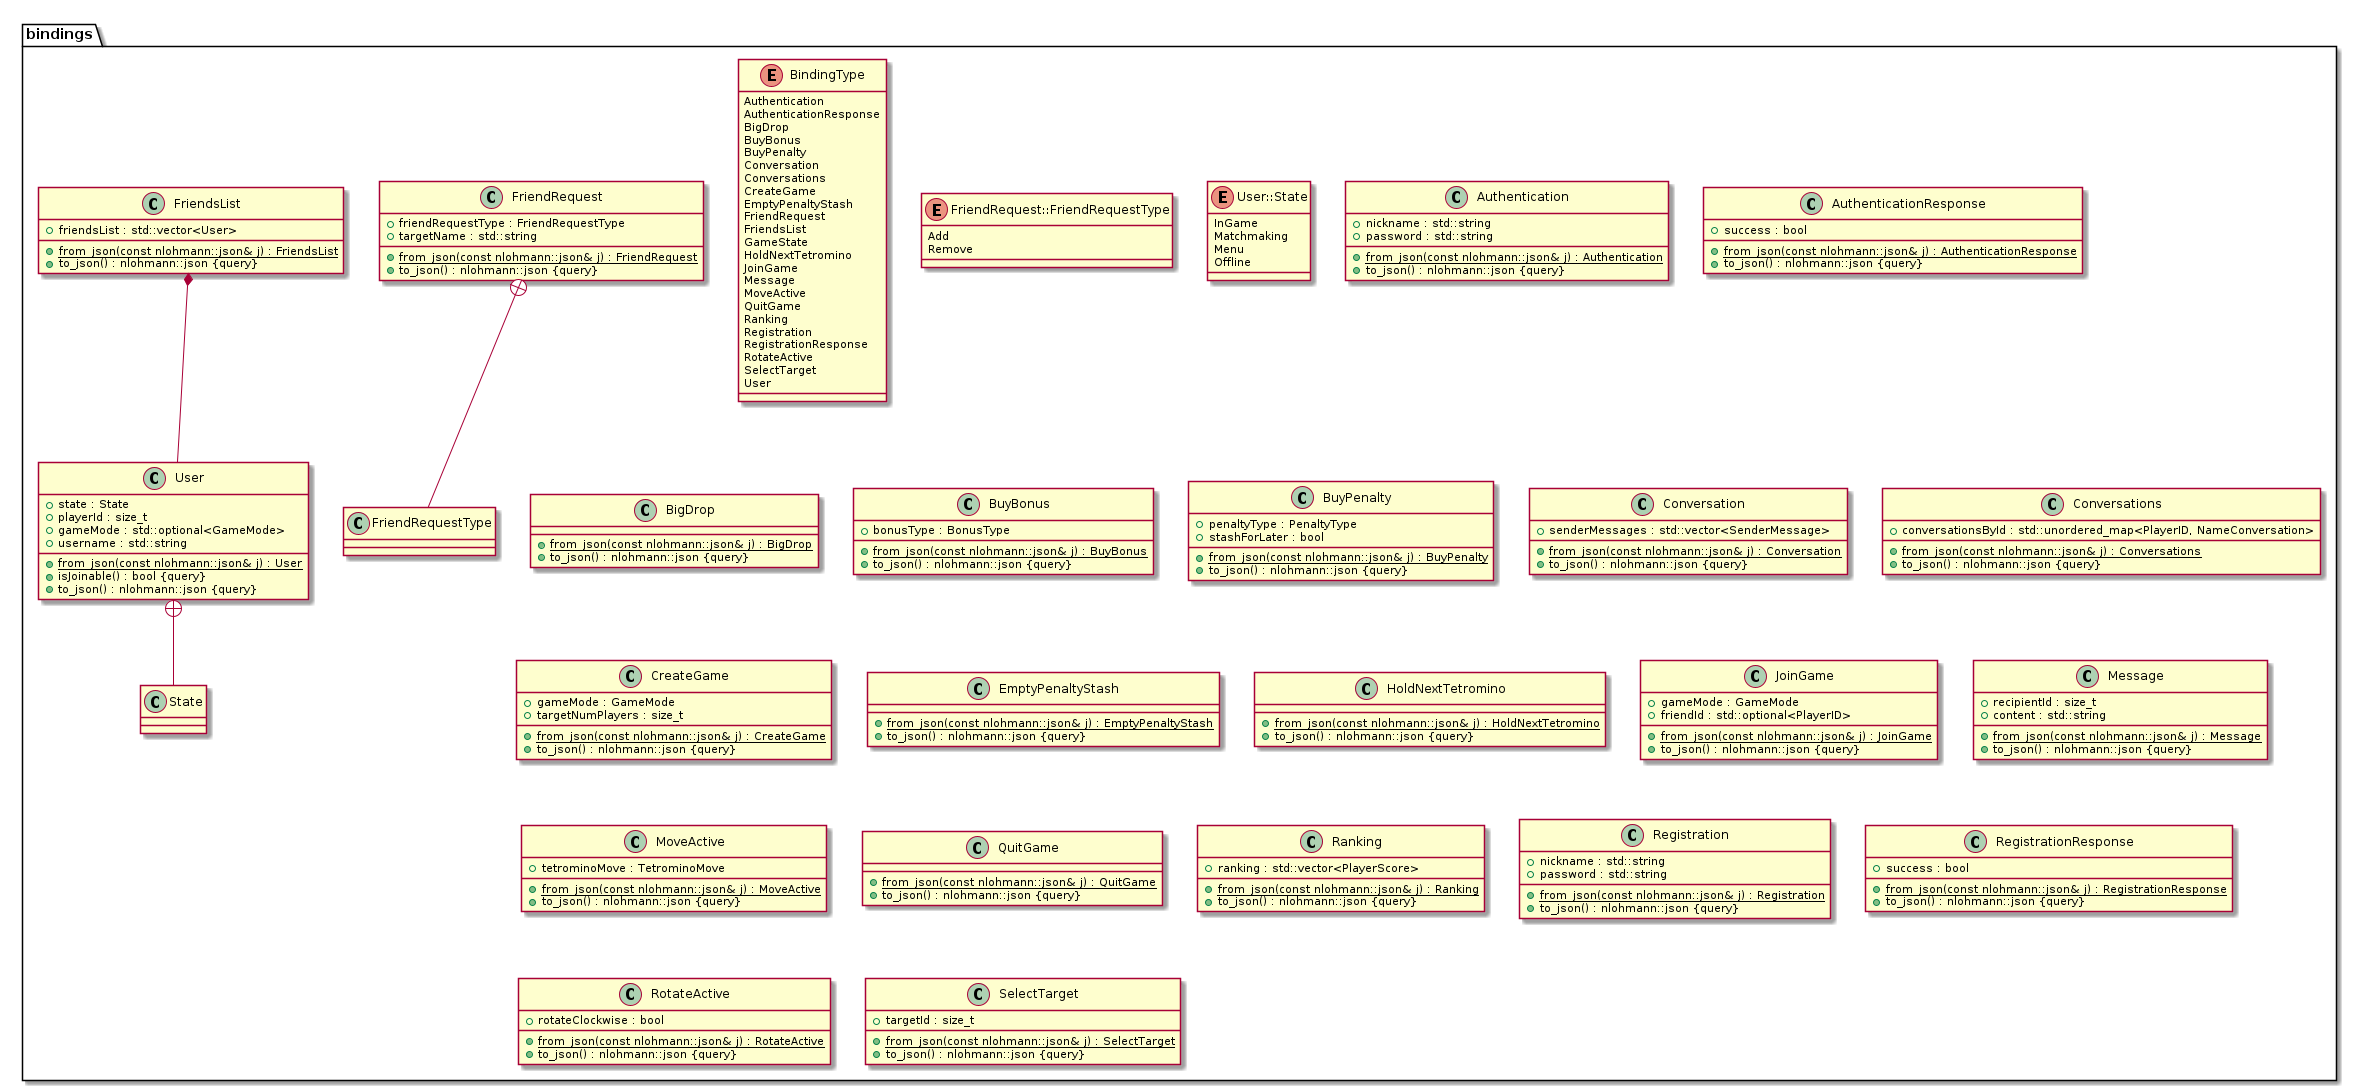
\includegraphics[scale=0.1, angle=90]{../../res/uml/class/BindingClass.png}
	 \caption{L'espace de nommage de \textit{bindings}}
	 \label{fig:BindingDiagram}
\end{figure}

\subsubsection*{Structure de Network}

Pour chaque utilisateur qui se connecte au réseau, une instance de ClientLink est créée avec son socket. Au fil de l'état de l'utilisateur, le ClientManager le rajoute ou non dans le vecteur d'utilisateur authentifiés.

Nous pouvons voir le ClientLink comme une classe pour transmettre les paquets reçus d'un utilisateur en question puis ClientManager les traite pour que le serveur prenne en compte un événement.

\begin{figure}[H]
	\centering
	 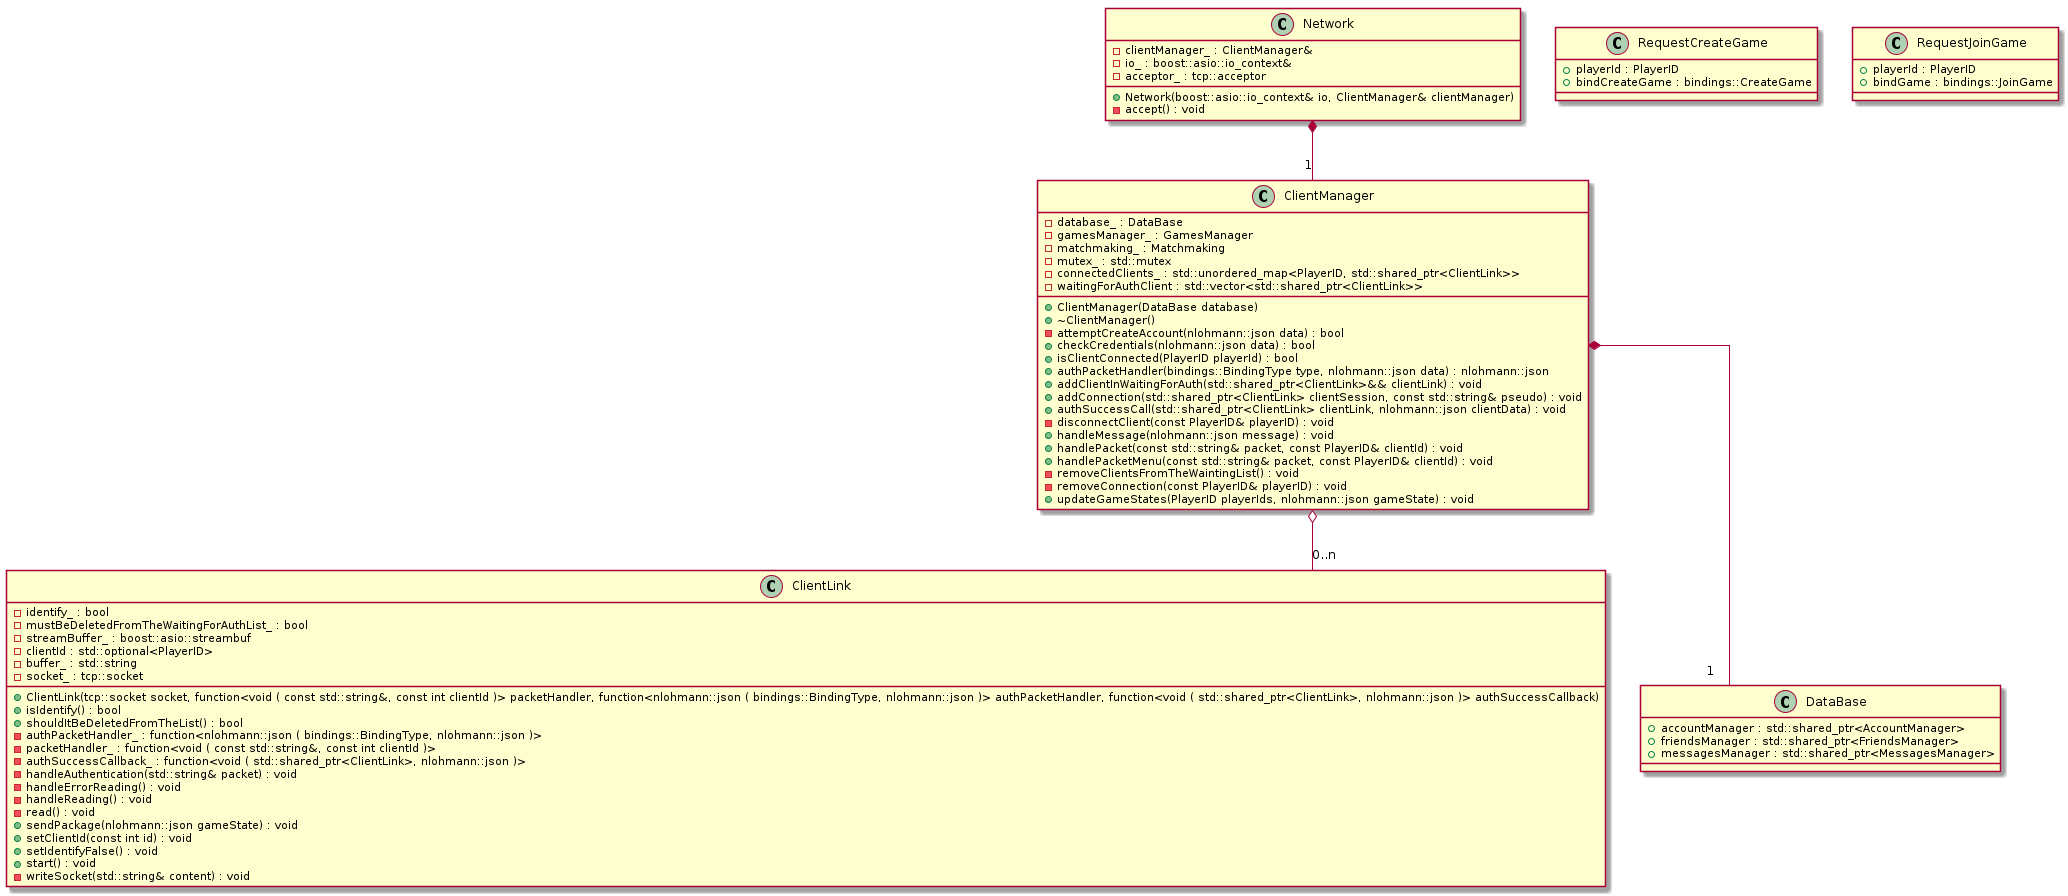
\includegraphics[scale=0.2]{../../res/uml/class/NetworkClass.png}
	 \caption{Diagramme de classes de Network}
	 \label{fig:NetworkDiagram}
\end{figure}

\subsubsection*{AccountService}

La classe AccountService permet de récuperer des informations dans la partie de la base de données qui s'occupe des comptes de l'application. En recevant des bindings précis, elle peut changer des champs dans la base de données ou vérifier les entrées données pour s'authentifier ou se connecter à un compte. 

\subsubsection*{SocialService}

La classe SocialService permet de récupérer des informations dans la partie de la base de données concernant les amis d'un compte donnée ou les messages existants entre deux comptes différents. Nous pouvons également faire des opérations dans la base de données avec des méthodes de la classe. \textit{ex. enlever un ami de sa liste d'amis}

\subsubsection{Le Matchmaking}
La classe Matchmaking est une classe que possède ClientManager. Elle est appelée quand ClientManager reçoit des paquets concernant une demande de création ou pour rejoindre une partie de jeu. Quand une demande de création de partie est dans le paquet, Matchmaking insère une nouvelle instance de GameCandidate dans un de ses attributs de gamesCandidate\textit{Mode de jeu}.\\
Pour GameCandidate, cela représente une partie en attente selon un mode de jeu sélectionné par le premier utilisateur, un nombre maximum d'utilisateurs, le nombre d'utilisateurs en train d'attendre. \\
Quand un nouveau utilisateur veut se rejoindre une possible partie en attente créée par un de ses amis ou aléatoirement, Matchmaking va chercher possiblement la partie en question et essayer de l'ajouter dans GameCandidate de cette dernière. Si le GameCandidate a atteint le quota de joueurs dans la partie en attente, Matchmaking appelle GamesManager dans une méthode privée pour lancer la partie en attente. 

\begin{figure}[H]
	\centering
	 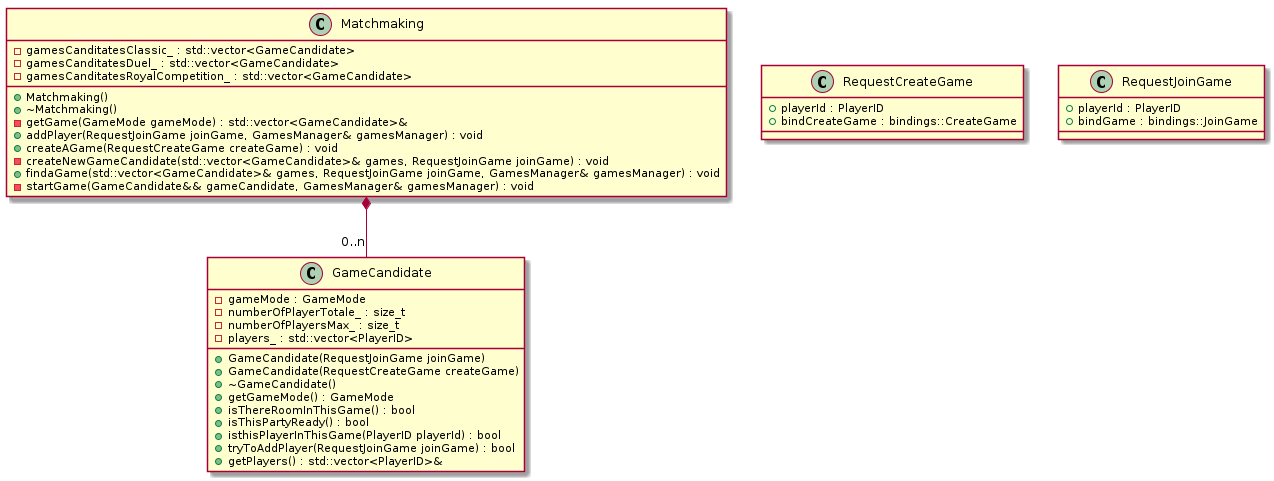
\includegraphics[scale=0.4]{../../res/uml/class/MatchMakingClass.png}
	 \caption{Diagramme de classes de Matchmaking}
	 \label{fig:MatchmakingDiagram}
\end{figure}

\subsubsection{GameServer}

la classe GamesManager contient plusieurs maps pour permettre de trouver le gameID et le gameServer correspondant, de même pour le gameID et le thread, et le PlayerID et le gameID. GamesManager crée des instances de GameServer quand Matchmaking l'appelle selon un mode de jeu et une liste de PlayerID de la partie créée. \\
Quand ClientManager reçoit un paquet pour le jeu avec un playerID, le paquet est envoyé à GamesManager et puis à GameServer avec enqueueBinding. GameServer le traite à son tick interne correspondant pour que le gameEngine puisse prendre en compte le paquet reçu du serveur. Quand toutes les demandes en attente durant la période de temps accordée sont traitées, le GameServer envoie le GameState changé à ClientManager. 

\begin{figure}[H]
	\centering
	 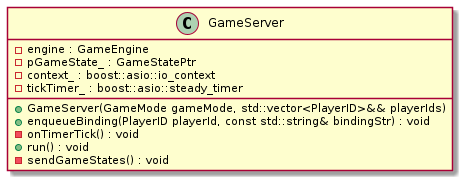
\includegraphics[scale=0.4]{../../res/uml/class/GameServerClass.png}
	 \caption{Diagramme de classes de GameServer}
	 \label{fig:GameServerDiagram}
\end{figure}

\subsubsection{MainServer}

La classe TetrisMainServer permet de lancer les instances tels que ClientManager, la base de données et DatabaseManager lorsqu'on lance le serveur avecou non le choix d'un port spécifique. 

\begin{figure}[H]
	\centering
	 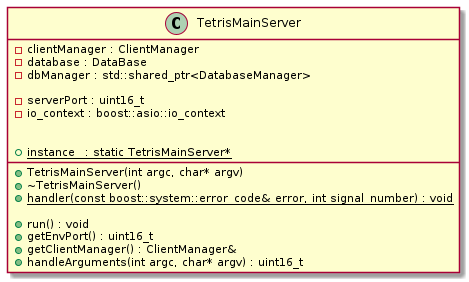
\includegraphics[scale=0.3]{../../res/uml/class/MainServerClass.png}
	 \caption{Diagramme de classe de TetrisMainServer}
	 \label{fig:GameServerDiagram}
\end{figure}

\subsubsection{Diagramme complet du serveur}

\begin{figure}[H]
	\centering
	 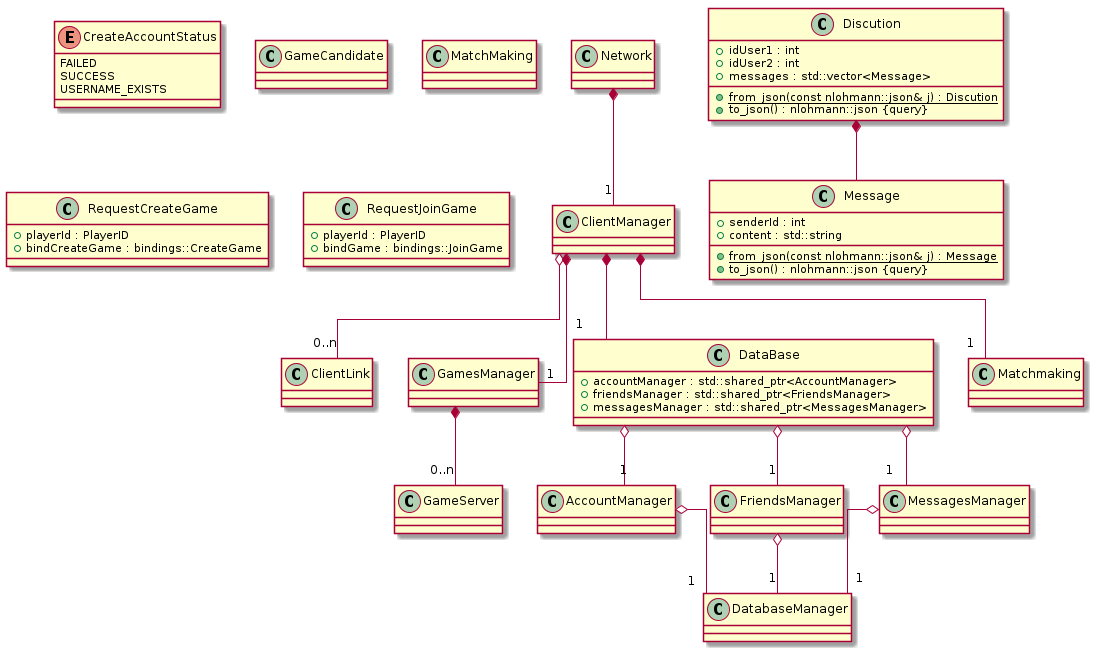
\includegraphics[scale=0.2]{../../res/uml/class/ServerStructureClass.png}
	 \caption{Diagramme de classes  simplifiées du Serveur}
	 \label{fig:WholeServerDiagram}
\end{figure}

\subsection{Architecture du client}

L'architecture du client possède plusieurs parties qui permettent de communiquer avec le serveur et de plus afficher les informations sur l'écran de l'utilisateur. Il possède également tous les éléments nécessaires pour avoir localement la logique de Tetris dans tous les modes.

\subsubsection{le Graphisme}

La disposition sur l'écran des informations reçues du serveur est séparée par les classes pour le graphisme et une classe MainTui ou MainGui selon le choix de l'utilisateur lors du lancement de l'application.

%\subsubsection*{les interfaces}

Pour le GUI et le TUI, nous avons suivi une architecture similaire pour chaque avec en commun l'utilisation de la classe abstraite AbstractGameDisplay. Cette dernière permet d'avoir une implémentation existante pour certaines fonctions qui extraient les informations du GameState. 

\begin{figure}[H]
    \centering
    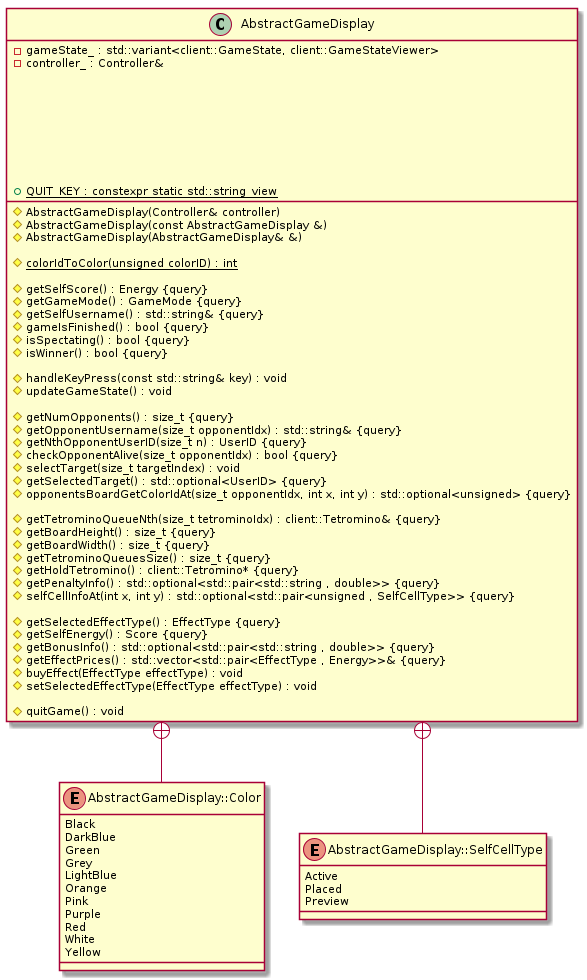
\includegraphics[scale=0.2]{../../res/uml/class/AbstractGameDisplayClass.png}
    \caption{Diagramme de classe de AbstractGameDisplay}
    \label{fig:InterfaceDiagram}
\end{figure}

\begin{figure}[H]
    \centering
    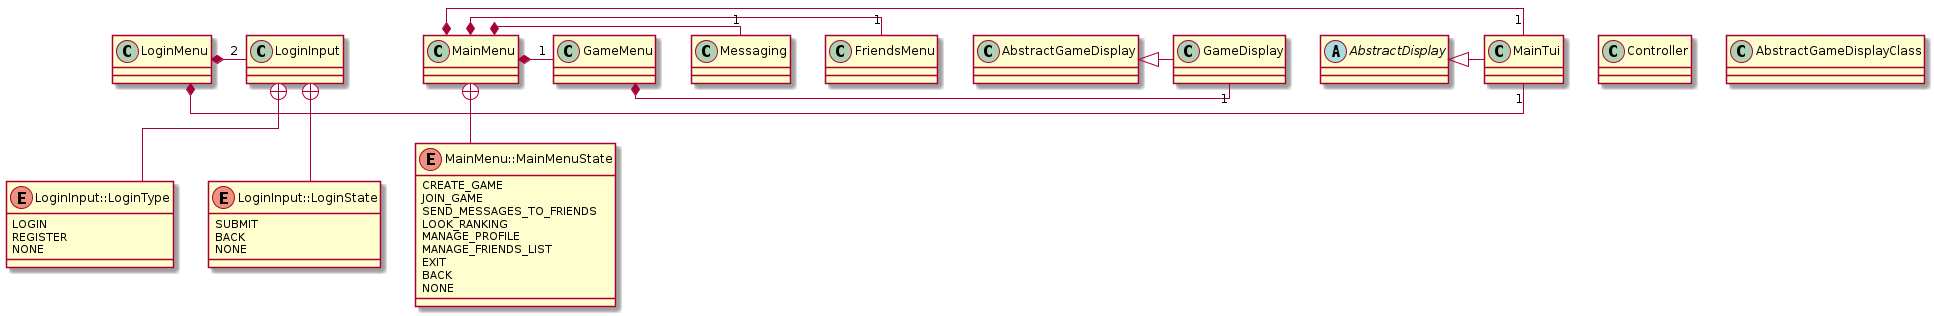
\includegraphics[width=1\textwidth]{../../res/uml/class/GraphismeStructureClass.png}
    \caption{Diagramme de classes des classes utilisées pour la partie graphique}
    \label{fig:GraphismeDiagram}
\end{figure}

\subsubsection{le NetworkManager}

La partie réseau du client est faite par la classe NetworkManager. Elle établit et met fin correctement la connexion avec le serveur. De plus, elle reçoit du serveur tous types de paquets et peut envoyer des paquets au serveur. Le traitement de ces paquets est fait dans une autre classe du client.

\begin{figure}[!ht]
	\centering
	 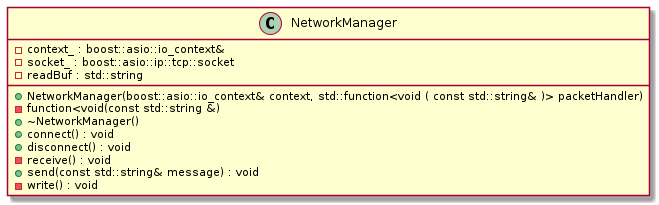
\includegraphics[scale=0.5]{../../res/uml/class/NetworkManagerClass.png}
	 \caption{Diagramme de classe de NetworkManager}
	 \label{fig:NetworkManagerDiagram}
\end{figure}

\subsubsection{le Controller}

Le Controller réunit la partie réseau et l'affichage des informations à l'utilisateur. Il possède une instance de chaque partie et d'autres informations que nous aurions besoin d'afficher à l'utilisateur (\textit{ex. la liste d'amis de l'utilisateur pour pouvoir lui afficher}). 

Le Controller permet également de traiter les paquets reçus de NetworkManager pour changer les informations que possède l'utilisateur jusque lors. Quand le client veut envoyer une information au serveur, le paquet est créé dans Controller et puis, NetworkManager l'envoie au serveur.

\begin{figure}[H]
	\centering
	 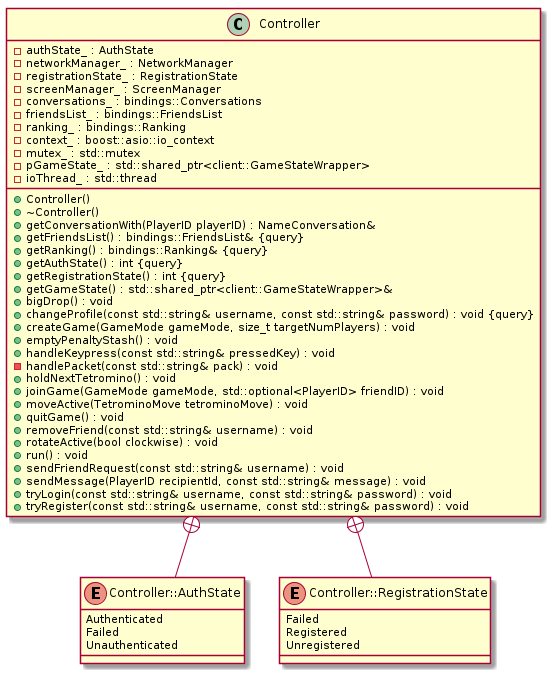
\includegraphics[scale=0.3]{../../res/uml/class/ControllerClass.png}
	 \caption{Diagramme de classe de Network}
	 \label{fig:ControllerDiagram}
\end{figure}

\subsubsection{Diagramme complet du client}

\begin{figure}[H]
	\centering
	 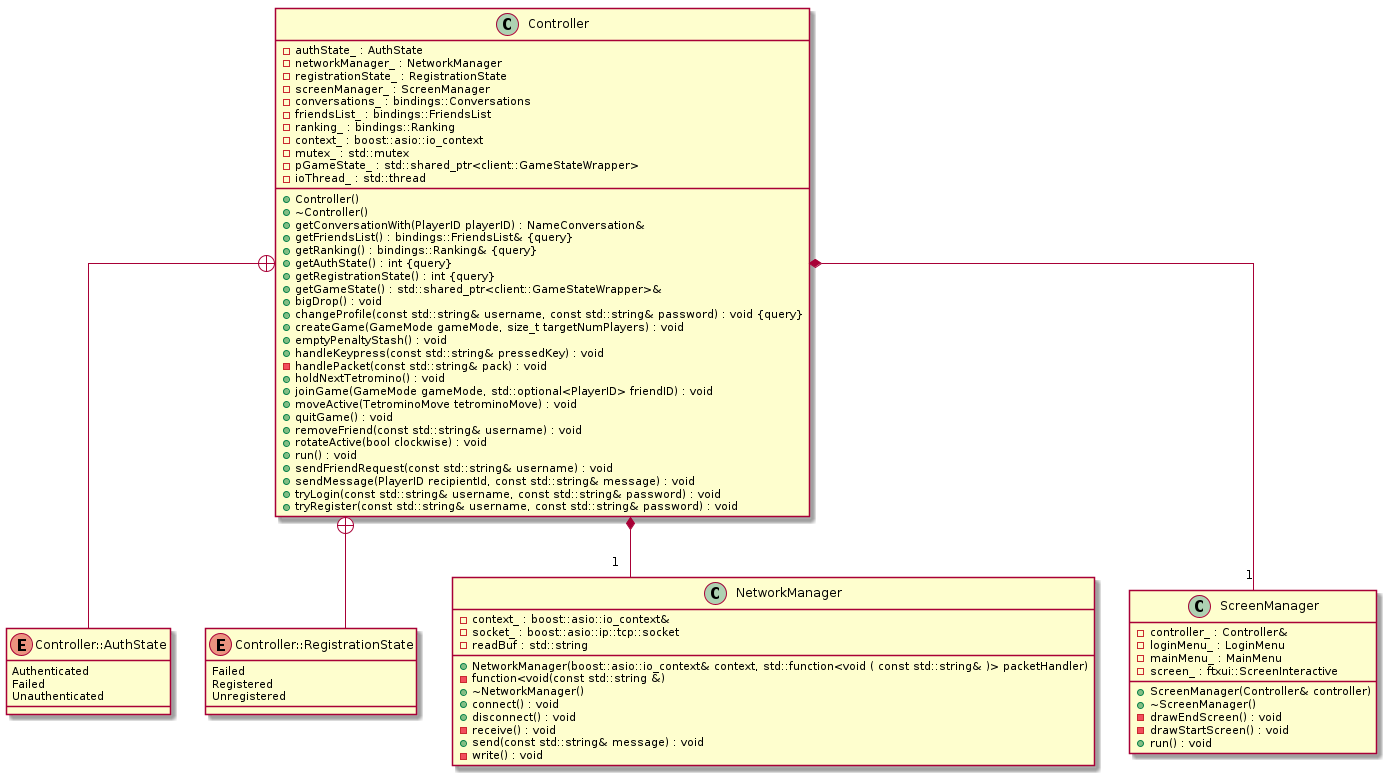
\includegraphics[scale=0.3]{../../res/uml/class/ClientStructureClass.png}
	 \caption{Diagramme de classes du client}
	 \label{fig:WholeClientDiagram}
\end{figure}

\newpage

\section{Fonctionnement du système}

\subsection{Création d'un compte}

Lors du lancement de l'application, si l'utilisateur n'a pas de compte, il commence la procèdure d'inscription. Le Controller va se connecter au réseau du serveur. Network va créer une nouvelle instance de ClientLink. Ce nouvel objet le notifie à ClientManager qui appelle ensuite une méthode interne à elle-même. Ensuite l'utilisateur va entrer un username et un mot de passe sur l'interface et validera l'action. Le Controller enverra les données dans un paquet au ClientLink correspondant à l'utilisateur. ClientManager traite le paquet une fois signalé par ClientLink. La réponse au succès ou non de la nouvelle entrée dans la base de données est transmise de ClientManager à ClientLink qui écrira la réponse dans le socket. Le Controller traite la réponse et changera l'attribut nécessaire pour savoir le status de l'utilisateur.

\begin{figure}[H]
    \centering
    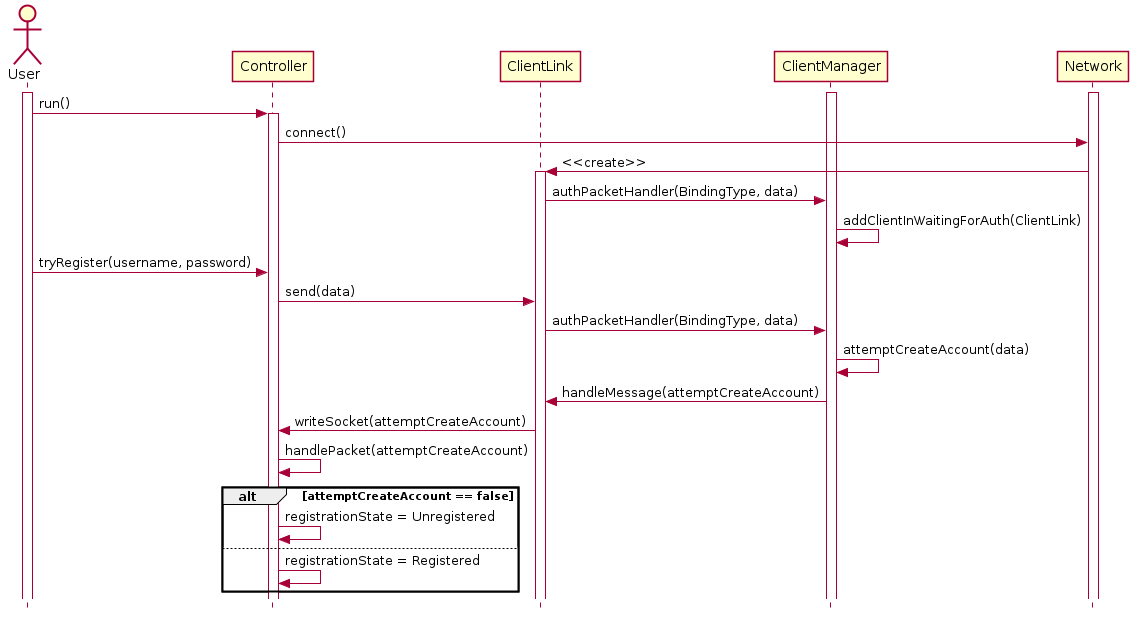
\includegraphics[width=1\textwidth]{../../res/uml/sequence/InscriptionSequence.png}
    \caption{Diagramme de séquence d'inscription}
    \label{fig:InscriptionDiagram}
\end{figure}

\subsection{Connexion}

Lors du lancement de l'application, si l'utilisateur possède déjà un compte, il commence la procédure d'authentification. Le Controller va se connecter au réseau du serveur. Network va créer une nouvelle instance de ClientLink. Ce nouvel objet le notifie à ClientManager qui appelle ensuite une méthode interne à elle-même. Ensuite l'utilisateur va entrer un username et un mot de passe sur l'interface et validera l'action. Le Controller enverra les données dans un paquet au ClientLink correspondant à l'utilisateur. ClientManager traite le paquet une fois signalé par ClientLink. ClientManager envoie un message à la base de données pour vérifier si le compte existe et si le mot de passe est correct avec le compte associé. La réponse sera récupérée par ClientManager. Ce dernier envoie un paquet à écrire pour le ClientLink de l'utilisateur. Le Controller traite la réponse et changera l'attribut nécessaire pour savoir le status de l'utilisateur.

Si l'authentification est un succès, le ClientManager va rajouter le ClientLink associé à l'utilisateur dans le vecteur d'utilisateurs connectés.

\begin{figure}[H]
    \centering
    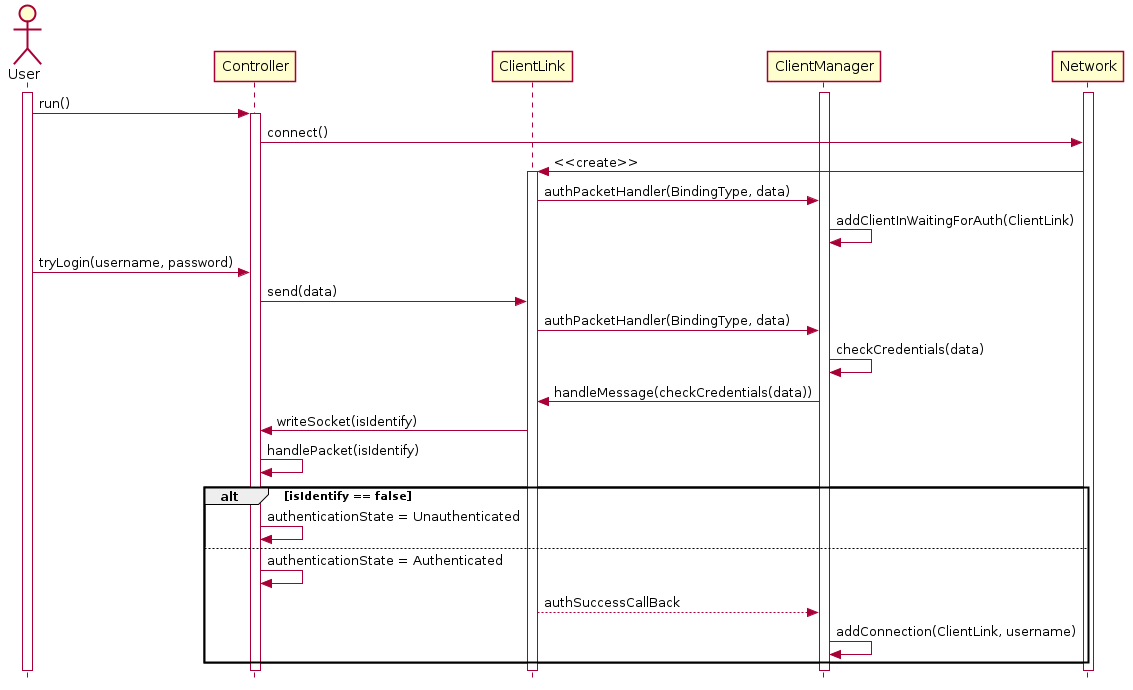
\includegraphics[width=1\textwidth]{../../res/uml/sequence/ConnexionSequence.png}
    \caption{Diagramme de séquence de connexion}
    \label{fig:ConnexionSeqDiagram}
\end{figure}

%\subsection{Menu du jeu côté serveur}
%
%\subsection{Menu du jeu côté client}

\subsection{Matchmaking côté serveur}

Quand l'utilisateur veut créer une partie, ClientLink reçoit un paquet correspondant à sa demande. Ce dernier est transmis à ClientManager avec l'userID du client. ClientManager traite la demande et va envoyer un message à Matchmaking pour créer une partie. Une instance de GameCandidate sera créée par Matchmaking en conséquent. 

Quand l'utilisateur veut rejoindre une partie existante, ClientLink reçoit un paquet correspondant à sa demande. Ce dernier est transmis à ClientManager avec l'userID du client. ClientManager traite sa demande et va envoyer un message à Matchmaking. Il va essayer de trouver selon le mode de jeu et la demande ou non de la présence d'un autre userID spécifique. Si la partie est trouvée, Matchmaking va essayer de rajouter l'utilisateur dans l'instance de GameCandidate. Si cela n'est pas possible, MatchMaking créera alors une nouvelle instance de GameCandidate. 

Puis quand le nombre de joueurs maximum dans la partie sera atteint, Matchmaking enverra un message à GamesManager pour initier une nouvelle instance de GameServer.

\begin{figure}[H]
    \centering
    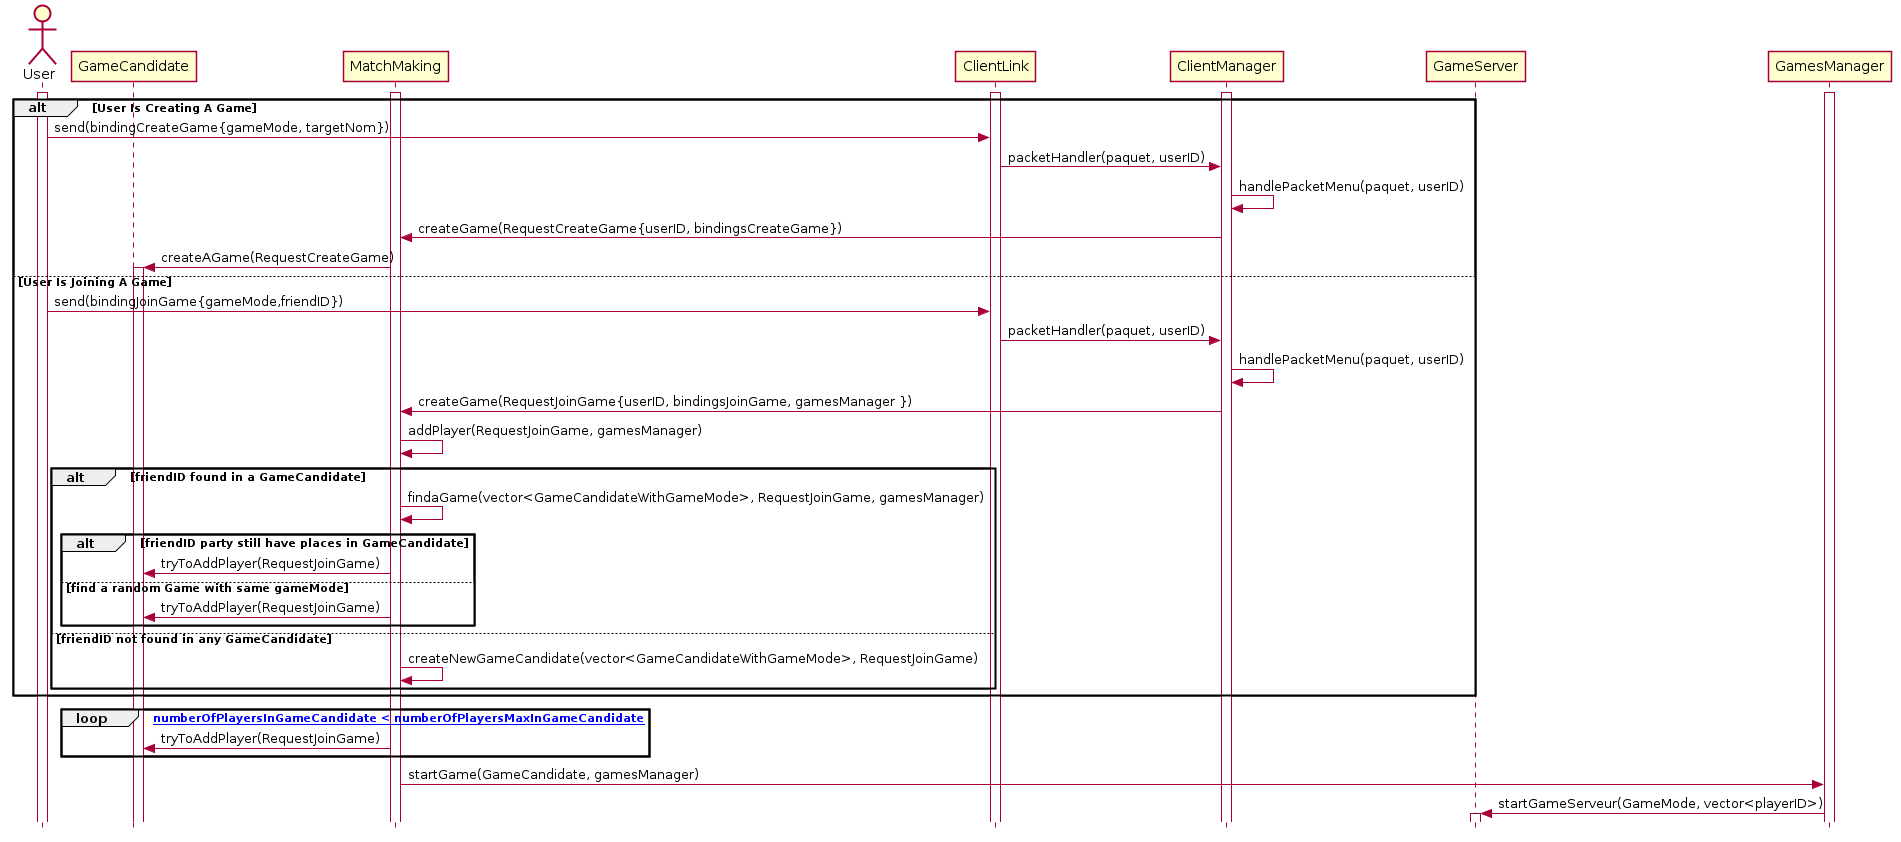
\includegraphics[width=1\textwidth]{../../res/uml/sequence/MatchMakingServerSequence.png}
    \caption{Diagramme de séquence de Matchmaking côté serveur}
    \label{fig:MatchmakingServerDiagram}
\end{figure}

\subsection{Matchmaking côté client}

Quand un utilisateur sélectionne dans le menu pour commencer une partie, il commence la procédure de Matchmaking. Le GameMenu s'affiche sur l'écran.

L'utilisateur peut créer une nouvelle partie de jeu. Il sélectionne le mode de jeu. Puis si ce n'est pas le mode Dual ou Endless, il doit remplir le champs concernant le nombre maximum de joueurs dans la nouvelle partie. Une fois que le GameMenu ait toutes ces informations, il envoit une requête à Controller, elle sera mise dans un paquet pour que NetworkManager l'écrive dans le socket du réseau. 

L'utilisateur peut également choisir de rejoindre une partie existante avec le mode de jeu souhaité. Il sélectionne une partie créée par un de ses amis en ligne ou rejoint une partie existante aléatoirement. Une requête est envoyée de GameMenu à Controller pour qu'un paquet soit transféré au serveur via le NetworkManager.

\begin{figure}[H]
    \centering
    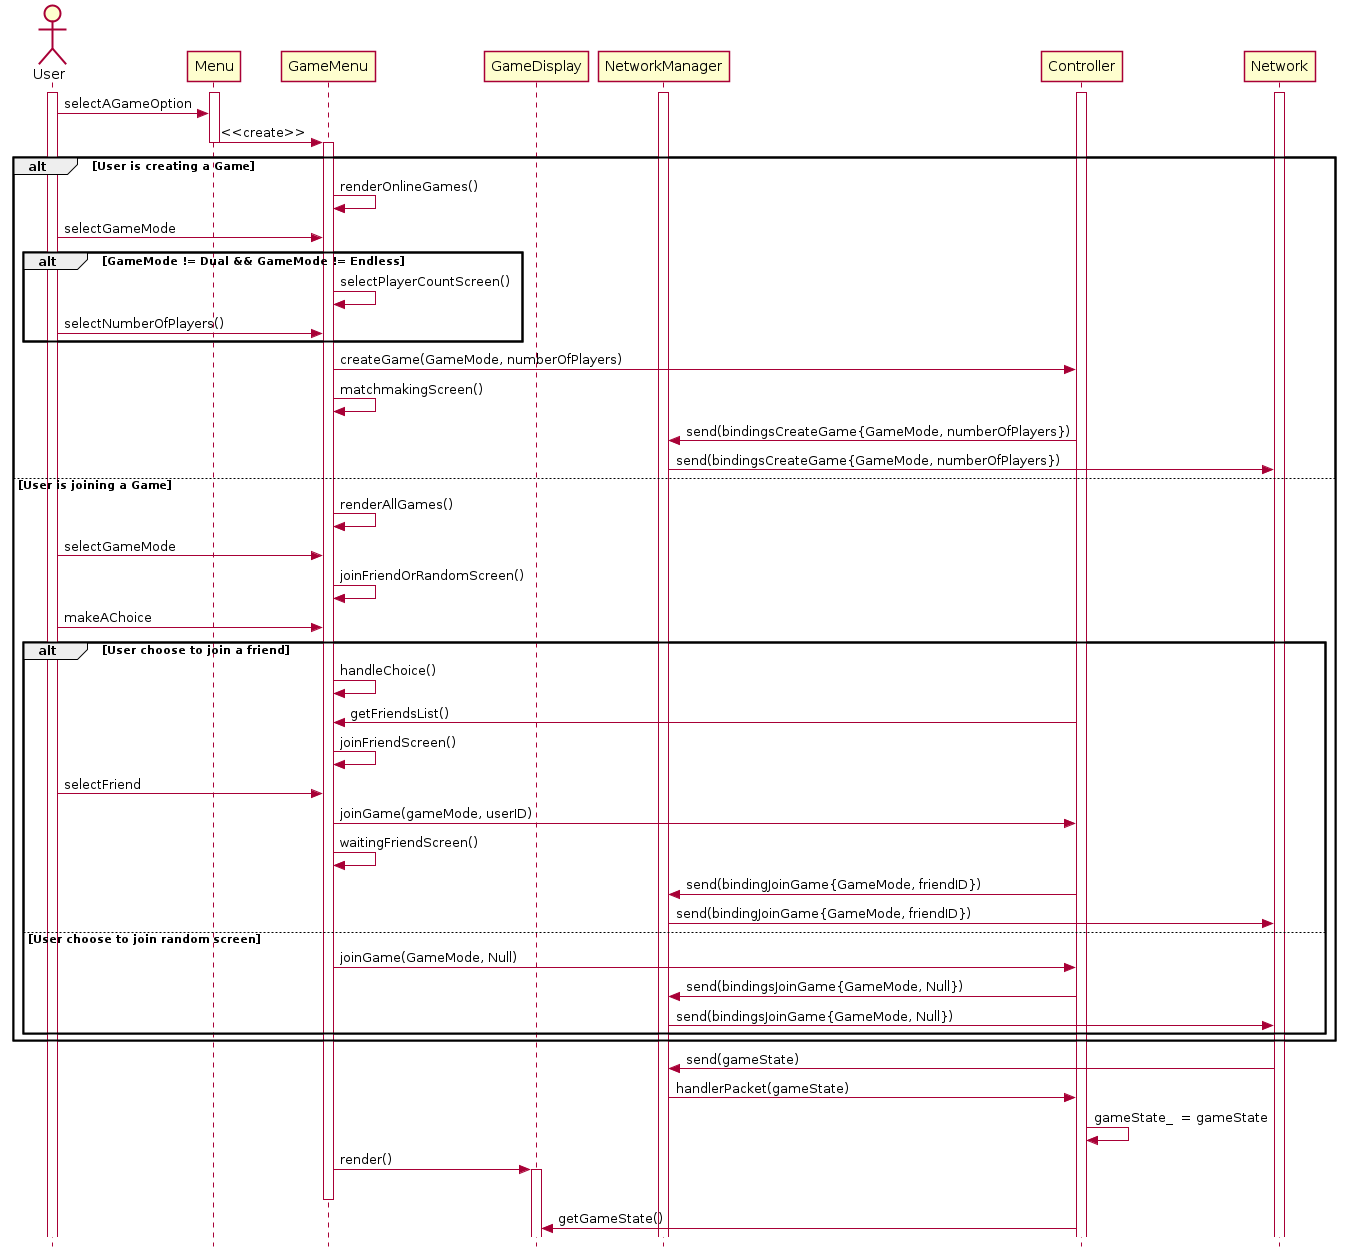
\includegraphics[width=1\textwidth]{../../res/uml/sequence/MatchMakingClientSequence.png}
    \caption{Diagramme de séquence de Matchmaking côté client}
    \label{fig:MatchmakingClientDiagram}
\end{figure}

\subsection{Game côté serveur}

Au début d'une partie, GamesManager commencera une instance de GameServer avec le mode de jeu indiqué et les playerID des utilisateurs présents. Durant la partie, le joueur enverra des paquets de jeu à son ClientLink correspondant. Ensuite, le paquet est reçue dans ClientManager puis transmis à GamesManager qui rajoutera à la queue de paquets que le GameServer doit encore traitée. Le GameServer traite le paquet et l'incorpore dans son GameEngine. Une fois tous les paquets reçsu traités, le GameServer envera le GameState de la partie mis à jour à ClientManager. Puis il est passé à ClientLink pour être écrit dans le socket afin que l'utilisateur le reçoive. A la fin d'une partie, le GameServer le signalera à GamesManager puis se détruit.

\begin{figure}[H]
    \centering
    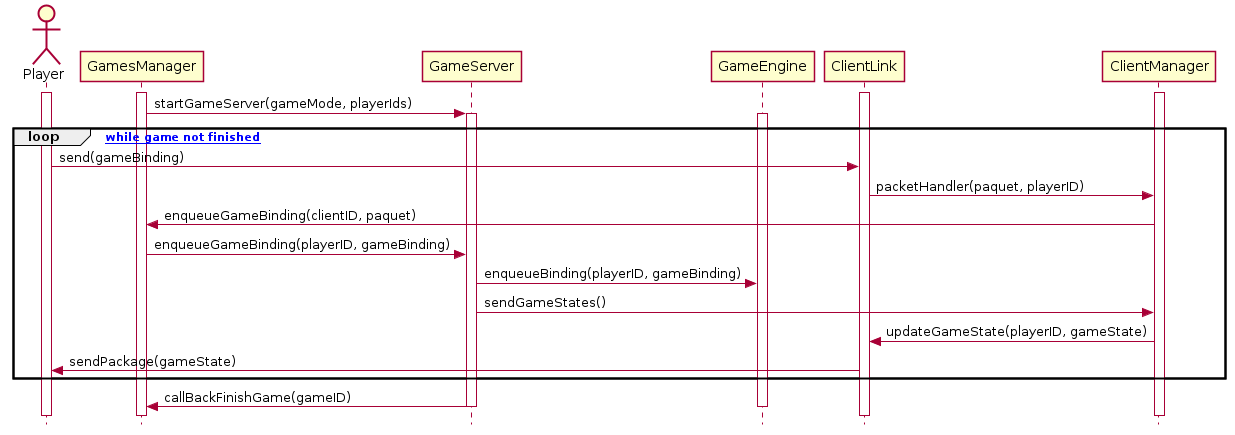
\includegraphics[width=1\textwidth]{../../res/uml/sequence/GameServerSequence.png}
    \caption{Diagramme de séquence du jeu côté serveur}
    \label{fig:GameServerSeqDiagram}
\end{figure}

\subsection{Game côté client}

Au début d'une partie, l'objet GameDisplay est activé. Durant la partie, le joueur presse une touche de son clavier qui sera signalé à GameDisplay. Ce dernier enverra un message à Controller qui sera transformé en paquet et écrit dans le socket à NetworkManager. Le paquet sera reçu au serveur. Une fois le paquet traité, le serveur enverra à NetworkManager le nouveau gameState de la partie dans un paquet. Ce dernier sera traité dans le Controller qui forcera l'écran de l'utilisateur de se refaire.

\begin{figure}[H]
    \centering
    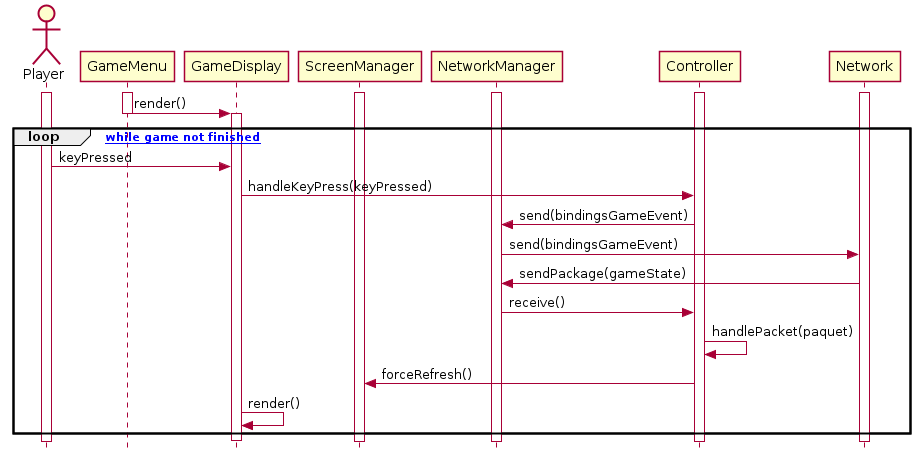
\includegraphics[width=1\textwidth]{../../res/uml/sequence/GameClientSequence.png}
    \caption{Diagramme de séquence du jeu côté client}
    \label{fig:GameClientSeqDiagram}
\end{figure}

%\subsection{Envoi d'une requête}

%\subsection{Traitement d'une requête}

%\subsection{Lancement d'une partie}

%\subsection{Rejoindre un Lobby}

\section{Annexes}

\subsection{Liens}

\href{Super Rotation System}{https://tetris.fandom.com/wiki/SRS}

\end{document}
